%Publication version
\documentclass[aps,twocolumn,prd,superscriptaddress,showpacs,nofootinbib,fixfloat]{revtex4}
%Draft version
%\documentclass[aps,prd,superscriptaddress,showpacs]{revtex4}
%\usepackage{doublespace}
\usepackage{graphicx}
\usepackage{dcolumn}
\usepackage{bm}
\usepackage{natbib}

%\topmargin+1cm

% Journals
\newcommand{\aaps}{{Astron.~Astrophys.~Supp.}}
\newcommand{\physrep}{{Physics~Reports}}
\newcommand{\araa}{{Annu.~Rev.~Astron.~Astrophys.}}
\newcommand{\aap}{{Astron.~Astrophys.}}
\newcommand{\apjl}{{Astrophys.~J.~Lett.}}
\newcommand{\apjs}{{Astrophys.~J.~Supp.}}
\newcommand{\aj}{{Astron.~J.}}
\newcommand{\mnras}{{Mon.~Not.~R.~Astron.~Soc.}}

% Making life easier
\newcommand{\be}{\begin{equation}}
\newcommand{\ee}{\end{equation}}
\newcommand{\bea}{\begin{eqnarray}}
\newcommand{\eea}{\end{eqnarray}}
\newcommand{\backten}{\!\!\!\!\!\!\!\!\!\!}

% useful symbols
\newcommand{\nhat}{\hat{\bf n}}
\newcommand{\kvec}{{\bf k}}
\newcommand{\edm}{\epsilon_{dm}}
\newcommand{\edmnow}{\epsilon_{dm,0}}
\newcommand{\sv}{\langle\sigma_Av\rangle}
\newcommand{\khat}{\hat{\bf k}}

% Fermi is usually italicized - use \Fermi\ for space after word
\newcommand{\Fermi}{{\slshape Fermi}}

% math functions, units
\newcommand{\Mpc}{{\rm ~Mpc}}
\newcommand{\sech}{{\rm ~sech~}}
\newcommand{\Tr}{{\rm ~Tr~}}
\newcommand{\threej}[6]{{\left( \begin{array}{ccc} #1 & #2 & #3 \\ #4 & 
   #5 & #6 \end{array} \right)}}

% Doug's units
\newcommand{\s}{{\rm ~s}}
\newcommand{\kms}{{\rm ~km/s}}
\newcommand{\g}{{\rm ~g}}
\newcommand{\cm}{{\rm ~cm}}
\newcommand{\km}{{\rm ~km}}
\newcommand{\mm}{{\rm ~mm}}
\newcommand{\mJy}{{\rm ~mJy}}
\newcommand{\Jy}{{\rm ~Jy}}
\newcommand{\MJy}{{\rm ~MJy}}
\newcommand{\MJypSr}{{\rm ~MJy~sr^{-1}}}
\newcommand{\JypSr}{{\rm ~Jy~sr^{-1}}}
\newcommand{\Hz}{{\rm ~Hz}}
\newcommand{\kHz}{{\rm ~kHz}}
\newcommand{\MHz}{{\rm ~MHz}}
\newcommand{\GHz}{{\rm ~GHz}}
\newcommand{\K}{{\rm ~K}}
\newcommand{\mK}{\rm ~mK}
\newcommand{\microK}{\mu{\rm K}}
\newcommand{\eV}{{\rm ~eV}}
\newcommand{\eVs}{{\rm ~eV/s}}
\newcommand{\keV}{{\rm ~keV}}
\newcommand{\MeV}{{\rm ~MeV}}
\newcommand{\GeV}{{\rm ~GeV}}
\newcommand{\TeV}{{\rm ~TeV}}
\newcommand{\pc}{{\rm ~pc}}
\newcommand{\kpc}{{\rm ~kpc}}
%\newcommand{\Mpc}{{\rm ~Mpc}}
\newcommand{\erg}{{\rm ~erg}}
\newcommand{\degree}{^{\rm o}}
\newcommand{\sigmav}{\langle\sigma_Av\rangle}
\newcommand{\zrock}{$Z_{\rm rock}$}
\newcommand\reftbl[1]{Table \ref{tbl:#1}}
\def\la{\vcenter{\hbox{$<$}\offinterlineskip\hbox{$\sim$}}}
\def\ga{\vcenter{\hbox{$>$}\offinterlineskip\hbox{$\sim$}}}


% Necessary for appendices
\newcommand{\lmax}{{l_{\rm max}}}
\newcommand{\lmaxtwo}{{l_{\rm max}^2}}
\newcommand{\lmaxthree}{{l_{\rm max}^3}}


\newcommand\dpf[1]{{\bf (DPF: #1)}}

\begin{document}


\title{Is the 130 GeV Line Real? \\
  A Search for Systematics in the Fermi-LAT Earth Limb Data}

\author{Douglas P. Finkbeiner}
%\email{dfinkbeiner@cfa.harvard.edu}
\affiliation{Institute for Theory and Computation,
  Harvard-Smithsonian Center for Astrophysics, 
  60 Garden Street, MS-51, Cambridge, MA 02138 USA} 
\affiliation{Center for the Fundamental Laws of Nature,
  Physics Department, 
  Harvard University, 
  Cambridge, MA 02138 USA}

\author{Meng Su}
\affiliation{Institute for Theory and Computation,
  Harvard-Smithsonian Center for Astrophysics, 
  60 Garden Street, MS-51, Cambridge, MA 02138 USA} 

\author{Christoph Weniger}
\affiliation{Max-Planck-Institut f\"ur Physik, 
  F\"ohringer Ring 6, 
  80805 M\"unchen, Germany}

%% Claims of a line are important and demand a careful search for
%% systematics.  Limb photons provide a reference spectrum and look a bit
%% fishy.  Need more data.
\begin{abstract} Our recent claims of a Galactic center
  feature in Fermi/LAT data at approximately 130 GeV have
  prompted an avalanche of papers proposing explanations
  ranging from dark matter annihilation to exotic pulsar
  winds.  Because of the importance of such interpretations
  for physics and astrophysics, the threshold for discovery
  is unusually high.  This requires not only additional
  data, but a thorough investigation of possible LAT
  systematics.  While we do not have access to the details
  of each event reconstruction, we do have information about
  each event from the public event lists and spacecraft
  parameter files.  These data allow us to search for
  suspicious trends that could indicate a spurious signal.
  In particular, the Earth limb photons provide a smooth
  reference spectrum for null tests.  We examine these
  events and find a marginally significant 130 GeV feature
  in a small subset of the data.  This raises concerns about
  the 130 GeV Galactic center feature, even though we can
  think of no plausible model of instrumental behavior that
  connects the two.  A modest amount of additional limb data
  would tell us if the limb feature is a statistical fluke.
  If the limb feature persists, it raises serious concerns
  about the Pass 7 processing of $E > 100$ GeV events.
\end{abstract}

\pacs{}

\maketitle


%%%%%%%%%%%%%%%%%%%%%% SECTION I %%%%%%%%%%%%%%%%%%%%%%%%%%%%%%%
%% Dark matter is cool.  Line is a smoking gun.  Theory says continuum is
%% much stronger for MSSM, but there a models where you would see the line
%% first, so we look.

%% Weniger found it first.  Su & Finkbeiner said it is off center and might
%% be two lines.

\section{Introduction}

The search for dark matter takes many forms: exploration of
its astrophysical properties, direct detection in
underground labs, and even collider signatures of WIMPs or
related
particles~\citep{Jungman:1995df,Bergstrom:2000,Bertone:2005,
Hooper:2007Review, 2012arXiv1205.4882B}.

For indirect direction, distinguishing the dark matter
signal from conventional astrophysics background is always a
challenging. Gamma-ray line emission is a long-sought
``smoking gun'' for dark matter annihilation, as no
plausible astrophysical background can produce such line
signature\footnote{although a narrow feature is possible
\citep[see][]{2012arXiv1207.0458A}}.  The line(s) could be
produced by dark matter decays or annihilations into two
photons, or two-body final states involving one photon plus
a Higgs boson, Z boson, or other neutral non-SM particle. We
were not optimistic, because in most models the branching
ratio to lines is loop suppressed relative to the continuum
emission, and one would have expected to see the continuum
first in e.g. MSSM models~\citep[e.g.][]{Bergstrom:1997}.
Although this theoretical prejudice led most previous
studies to focus on continuum searches, this is not true in
all models that allow high line to continuum
ratios~\citep[e.g.][]{Bergstrom:1998, Bergstrom:2000,
Bertone:2009, Jackson:2010, Cline:2012, Weiner:2012}.  In
this work, we drop all theoretical prejudice and simply ask
if there is a line in the Galactic center spectrum.

The first claim of a line around 130 GeV emerged from the
work of Weniger~\citep{Weniger:2012}, which grew out of an
earlier search for other hard photon signals from
annihilations~\citep{Bringmann:2012}.  Weniger focused on
spectral fitting to photon events in regions of interest
designed to maximize S/N.  He found a 4.6$\sigma$
(3.2$\sigma$ after the trials factor correction) line
structure at 130 GeV .

Subsequent work by Su \& Finkbeiner approached the problem
with template fitting, assuming various profiles (Einasto,
NFW, Gaussian) for the DM distribution~\citep{linepaper}.
If the template is correct, this should allow extraction of
the DM signal with higher S/N.  This work found 6.6$\sigma$
(5.1$\sigma$ after the trials factor correction) for an
Einasto profile centered $1.5\degree$ west of the Galactic
center, and also suggest that there may be two lines, at
about 111 and 129 GeV.  The lower energy is tantalizing
because it matches the expected energy of a $Z\gamma$ line
if the higher energy is the $\gamma\gamma$ line.  Recent
evidence for lines at 111 GeV and 129 GeV with a local
significance of $3.3\sigma$ from Fermi unassociated point
sources provide further compelling support for the
hypothesis that the Galactic center line signal is indeed
from dark matter annihilation~\cite{doubleline}.

These papers have provoked theorists to try to reconcile the
observations with a number of theories~\citep{Dudas:2012,
Choi:2012, Kyae:2012, Lee:2012, Rajaraman:2012,
Acharya:2012, Garny:2012, Buckley:2012, Chu:2012, Kang:2012,
Buchmuller:2012, Heo:2012, Park:2012, Tulin:2012,
Cline:2012, Weiner:2012}.  But all of this work depends on
the question:

(What was the question?)



\section{The 130 GeV excess}
%%%%%%%%%%%%%%%%%%%%%% SECTION II %%%%%%%%%%%%%%%%%%%%%%%%%%%%%%%
In this section, %we focus on Galactic Center observations.
we introduce of some basic parameters and give a short
summary of the standard survey strategy of Fermi. We will
ask the question whether observations of the Galactic center
are peculiar in a way that could enhance instrumental
effects towards this direction and search for suspicious trends in
other regions of the sky and the reconstruction parameters.

%% Rock angle is 50, orbit precesses in 55 days, leading to nearly uniform
%% exposure.  Occasional ToO observations.


\subsection{Standard survey strategy and definitions}
\label{sec:conventions}
%% A. Standard survey strategy

%%   Define parameters (See table)

%%   Discuss standard events selection.

%% B. Peculiarities of the Galactic center observation

%%   we consider 3 ways to get a spurious signal

%%   1.  Incidence angles of Galactic Center observations
%%       The orbit / scan strategy impose certain patterns on (theta,phi)
%%       just from geometry.  If there are instrumental artifacts for such
%%       events, they could map disproportionately on to the GC.

%%       We choose events at those phi values away from the GC and find no
%%       excess of events near 111 or 130 GeV.  (Figs 2,3)

%%   2.  The Galactic center is bright
%%       Because the center is bright, a flaw in the instrument / data
%%       reduction that maps events to 130 GeV might only be noticed in a
%%       bright region of the sky.  However, we have other regions (limb,
%%       plane) that have lots of photons, and we see now 130 GeV excess in
%%       those samples.

%%   3.  The Galactic center has a hard spectrum
%%       Perhaps events could be mis-reconstructed, mapping events down
%%       from higher energy.  However, there are not even enough events
%%       above 300 GeV to explain the signal, even if all of them got
%%       mapped to 130 GeV.

\begin{table*}
  \begin{center}
    \begin{tabular}{lcrrcl}
      \hline
      Parameter &\hphantom{i}& & Range &\hphantom{i}&  Description\\
      name      && min & max &&            \\
      \hline
      $\theta$ &&    0 &  $\sim80$ && Polar coordinate (instrument frame) \\
      $\phi$   &&    0 &       360 && Azimuthal coordinate (instrument frame) \\
      $(x,y,z)$&&  $-1$& $1$ && Cartesian coordinates;
      $\propto(\sin\theta\cos\phi, \sin\theta\sin\phi, \cos\theta)$\\
      $Z$      &&    0 & $\sim113$ && Zenith angle (horizon at $Z=113\degree$) \\
      $\ell$   &&    0 & 360 && Galactic longitude \\
      $b$      &&  -90 &  90 && Galactic latitude \\
      $\psi$   &&    0 & 180 && Angle to Galactic center; $\cos\psi=\cos\ell\cos b$ \\
      \zrock\  && -110 & 110 && Rocking angle (boresight angle N of zenith) \\
      \hline
    \end{tabular}
    \caption{Event parameter definitions. The Cartesian coordinates $(x, y, z)$ are
    defined such that the $z$-axis corresponds to the LAT boresight, and the
    y-axis is parallel to the solar panels.}
    \label{tab:parameters}
  \end{center}
\end{table*}

We have defined the relevant event parameters used in this
paper in Tab.~\ref{tab:parameters}: $\theta$ is the
reconstructed incidence angle of the photon event with
respect to the LAT boresight -- defined as the $z$-axis
while the $y$-axis is parallel to the solar panels; $\phi$
is the reconstructed incidence angle with respect to the
$+y$ axis (the normal to the $y-z$ plane with positive
defined as facing the Sun, or along the orbiting velocity
vector). The Zenith angle $Z$ is defined as the angle
between the reconstructed event direction and the zenith
line, which is connecting the Earth center with the
satellite center.  Lastly, \zrock\ is the rocking angle of
the satellite (the the boresight angle north of the zenith)
at the time of the event.  All angles are in units of
degrees. 
% EARTH_AZIMUTH_ANGLE (degrees)

\begin{table*}
  \begin{tabular}{lllccc}
    \hline
    `Region' &&Cuts & $N(>100\GeV)$ & $\frac{N(>100\GeV)}{N(>30\GeV)}$ & $\frac{N(>300\GeV)}{N(>100\GeV)}$\\
    \hline
    Standard events      &  & $Z<100^\circ$ & 5093 & 13.4\% & 9.6\% \\
    Inner Galactic plane &  & $Z<100^\circ$, $3^\circ < |\ell| < 30^\circ,\ |b|<2^\circ$     & 703 & 16.9\% & 9.8\% \\
    Galactic center      &  & $Z<100^\circ$, $\psi<3^\circ$ & 82 & 17.4\% & 9.8\% \\
    Galactic center line &  & $Z<100^\circ$, $\psi<3^\circ$, $120\GeV<E<138\GeV$             & 26 & -- & -- \\
    Earth limb           &  & $Z>110^\circ$ & 3120 & 10.2\% & 9.2\% \\
    Earth limb line      &  & $Z>110^\circ$, $30^\circ<\theta<45^\circ$, $120\GeV<E<138\GeV$ & 45 & -- & -- \\ 
    % FWHM of GC line is 13.6%
    \hline
  \end{tabular}
  \caption{Different sets of events that we use throughout this work. In
  addition, we show the total number of events and event ratios.
  We always restrict the events to $>10\GeV$.}
  \label{tab:regions}
\end{table*}

In Tab.~\ref{tab:regions} we define some key sky and
paramter regions %(cuts on the full set of events)
that we will use
throughout this work: `Standard events' are all events with
the zenith angle cut $Z<100^\circ$ recommended by the LAT
team, which
avoids contamination with the Earth limb photons (see
Section~\ref{sec:EarthLimb}); `Inner Galactic plane' refers to a part of the
Galactic disk close to but without the center;
`Galactic center' events are defined as coming from within
a radius of
$3^\circ$ around $\ell=b=0^\circ$; `Earth limb events' are
defined as all events with zenith angles $Z>110^\circ$, and
completely dominated by photons generated in CR interaction
with the atmosphere. `Line' events refer to subsets
with energies between $120$ and $138$ GeV. This energy range
is selected since the dominant line at the GC is found to be
around 129 GeV~\cite{linepaper}, and the FWHM of the line is
about 13.6\%~\cite{Weniger:2012}.

Throughout, we will use \texttt{P7CLEAN\_V6} events from 4
Aug 2008 to 18 Jul 2012, with the good-time-interval cuts
\texttt{DATA\_QUAL==1} and \texttt{LAT\_CONFIG==1}, however
without commonly adopted cut on the rocking angle
$|$\zrock$|<52^\circ$, unless stated otherwise. This last cut would remove
all low incidence angle Earth limb events.
% Contamination due to neglected rocking angle cut (GC
% events from zrock>52 etc?) What happens for P7SOURCE_V6?
\medskip

In \emph{standard survey mode}, the LAT points at zenith
angle \zrock\ offset north from the zenith perpendicular to
the orbit and \zrock\ south of the zenith (the opposite side
of the orbital plane) on the next, surveying the northern
and southern hemispheres on each orbit. The survey mode are
performed with a repeating pattern of slews with 17
waypoints about the velocity vector, the waypoint defines
the time and the corresponding angle at which the LAT
boresight is rocked north (on one orbit) or south (on the
other orbit) of the orbit plane\footnote{The survey mode can
be also performed with alternate explicit slew
commands}\footnote{The survey pattern profiles are available
at
\url{http://fermi.gsfc.nasa.gov/ssc/observations/types/allsky/}.
The effective dates and times for each profile are provided.
}. \zrock\ was $35\degree$ since the start of the nominal
mission on August 4, 2008 to May 7th, 2009, but was changed
to $50\degree$ on Sep 3rd, 2009 for better thermal
management of the downward-facing battery
radiator\footnote{Different observatory sky-survey profiles
with rocking angle 39$\degree$, 40$\degree$, and 45$\degree$
respectively have been tested with relatively short periods,
including the 3 orbit profile test for various rocking
angles.}. This rocking profile, combined with the precession
of the orbit every $\sim$55 days, allows the LAT to cover
the whole sky every two orbits with the most uniform sky
coverage in a short time.

This survey mode is only occasionally interrupted for
pointed observations of targets of opportunity (ToOs). The
total amount of time in the pointed observations is $<$20\%
of the total observing time. Fermi's survey observations are
regularly interrupted during passages through the South
Atlantic Anomaly. This interruption results in an exposure
differential between north and south of ~15\%. In addition,
sky-survey is occasionally interrupted by Autonomous
Repoints of the observatory for the purpose of triggered
gamma-ray bursts follow up observations.  \medskip

\begin{figure}[h]
  \begin{center}
    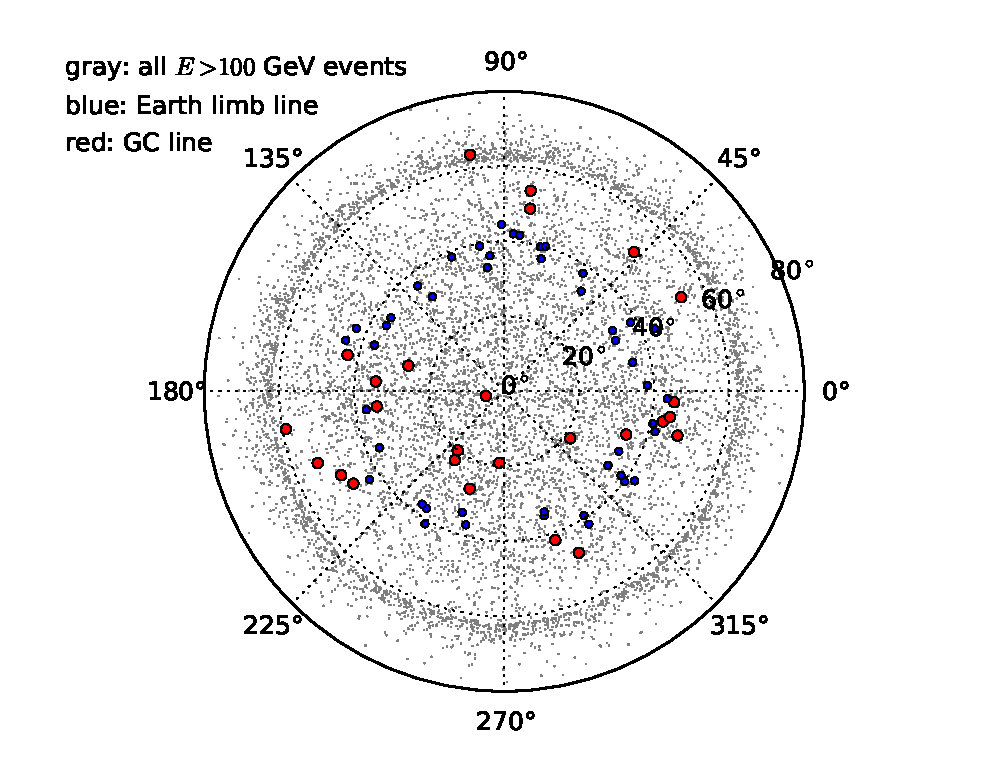
\includegraphics[width=0.9\linewidth]{plots/polarCounts.eps}
    \vspace{-0.5cm}
  \end{center}
  \caption{Incidence angle distribution of \emph{all} events
  with $E>100\GeV$ that enter our analysis (gray dots; see
  discussion in Sec.~\ref{sec:conventions}), of GC line
  events (red dots; see Tab.~\ref{tab:regions}) and of
  suspicious Earth limb events (blue dots; see
  Tab.~\ref{tab:regions} `Earth limb line'), as function of
  the instrumental coordinates $\theta$ and $\phi$. The
  Earth limb contribution is clearly visible in the gray
  dots at $\theta > 61^\circ$.}
  \label{fig:phiThetaDist}
\end{figure}

Due to the large rocking angle of \zrock$\simeq50\degree$
since September 2009, photons from the Earth limb (seen
under zenith angles of $Z\sim113^\circ$; see discussion
below) entered the FOV of the LAT. In
Fig~\ref{fig:phiThetaDist}, the gray dots show the
distribution of \emph{all} events (i.e.~without $Z$ cut)
with energies above 100 GeV as function of the instrumental
incidence polar and azimuthal angles $\theta$ and $\phi$.
The contribution from the Earth limb is clearly visible at
$\theta>60^\circ$. For comparison, the red and blue dots
show the `GC line' and the `Earth limb line' events that
will be discussed below.

\subsection{Peculiarities of the Galactic center observation}
The fact that the dominant 130 GeV line signal is near the
Galactic center raises a number of concerns.  The gamma-ray
flux at the GC is somewhat brighter and might have a harder
spectrum than neighboring regions. Also, the GC is near the
ecliptic ($\beta \approx -5\degree$) and may be observed in
a restricted range of angles in instrument coordinates
$(\theta, \phi)$ when the Sun passes near it.  We consider
whether these facts could exacerbate any systematic errors
in the LAT data to produce a spurious signal.

\subsubsection{Hypothesis: The Galactic center is bright, so
instrumental artifacts are more significant there}

\begin{figure}
  \centering
  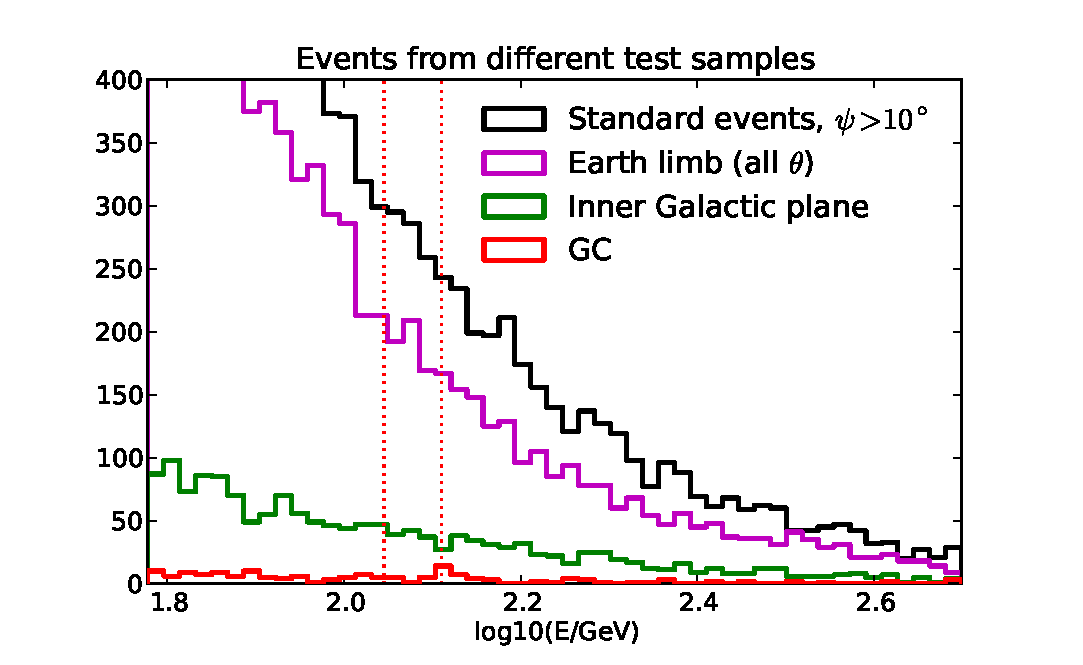
\includegraphics[width=1.0\linewidth]{plots/target_spectra.eps}
  \caption{Energy distribution in various bright regions as
  discussed in the text. None of them show the excess events
  around 130 GeV seen in the Galactic center. The red dotted
  lines indicate 111 and 129 GeV.}
  \label{fig:target_spectra}
\end{figure}

On a typical day, the hardware trigger rate of the LAT is
about $10^3$--$10^4\Hz$, whereas the rate of actually
accepted SOURCE and CLEAN class events is below
$3\Hz$~\citep{1206.1896}, the rate of $>100\GeV$ events
being even much lower. In light of these low trigger rates
(and assuming steady sources and CR background fluxes) it
would be surprising if the instrumental response of the LAT
would depend on the brightness of observed region.  However,
a few other bright regions exist besides the Galactic
center, and we check whether they show indications for
suspicious features at 130 GeV. The most important are the
Earth limb (with \emph{all} impact angles) and the inner
Galactic plane, see Tab.~\ref{tab:regions}; another region
with high statistics is just the whole set of standard
events excluding the region around the GC ($\psi>10^\circ$).
These targets provide a large number of high energy photons
that can be used to check for systematic artifacts in the
energy spectra.  We show the corresponding energy
distributions in Fig.~\ref{fig:target_spectra}. None of the
regions exhibit an $\mathcal{O}(1)$ excess at 130 GeV as
observed in the Galactic center. Note that in the vicinity
of the bright point sources Vela and Geminga (within
$0.8^\circ$, corresponding to $95\%$ containment angle of
the PSF) only four $>100\GeV$ events were measured (at
102.5, 111.5, 123.8 and 205.5 GeV), which makes them less
interesting for a systematic study.

\begin{figure*}
  \centering
  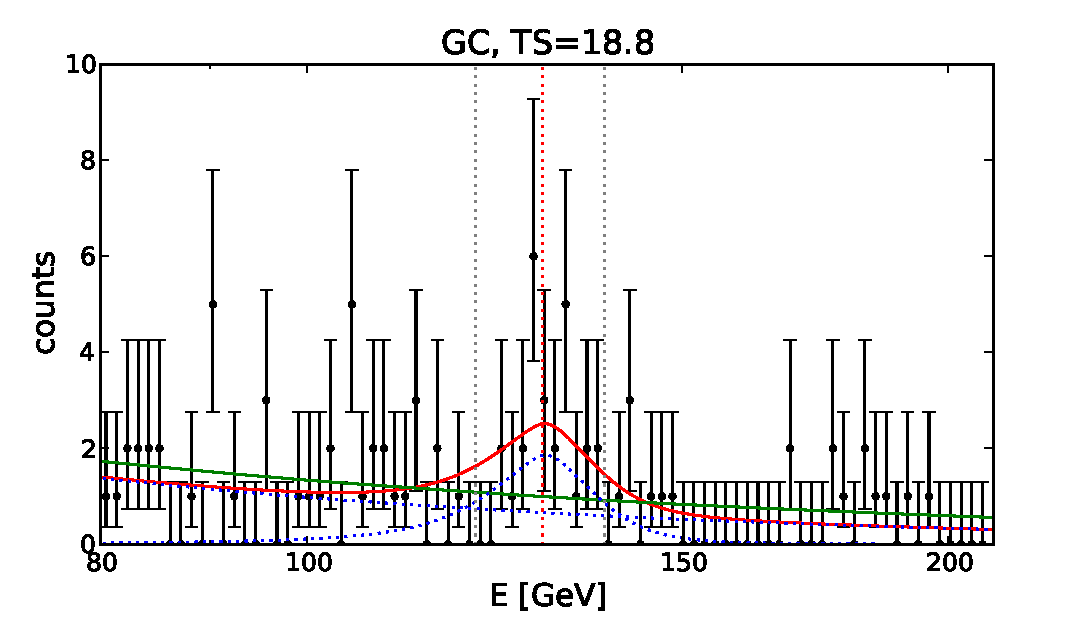
\includegraphics[width=0.48\linewidth]{plots/counts_GC.eps}
  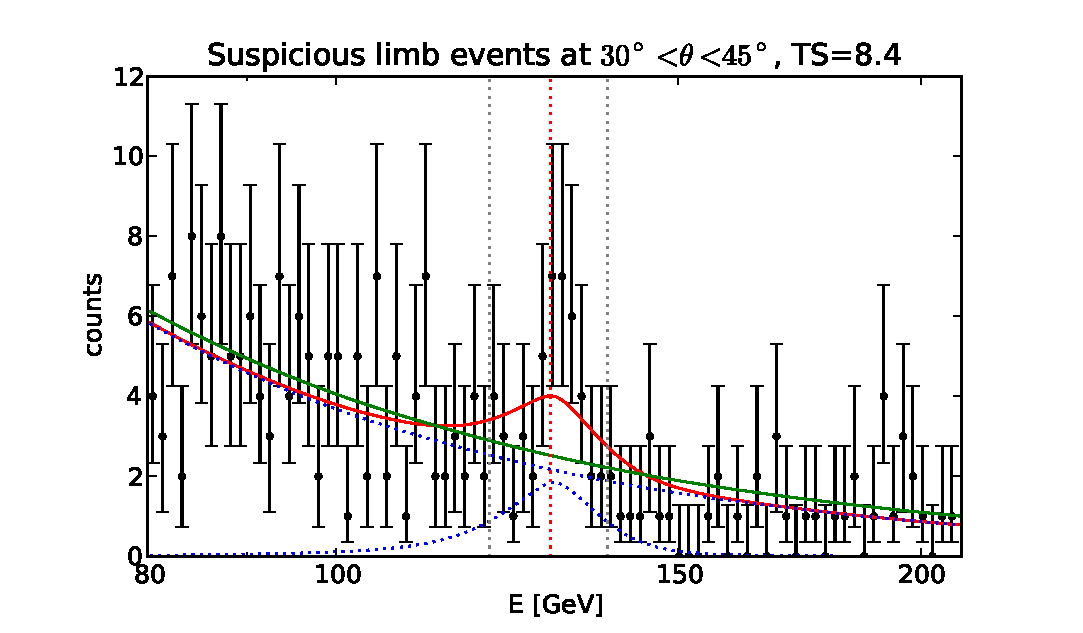
\includegraphics[width=0.48\linewidth]{plots/counts_suspiciousLimb.eps}
  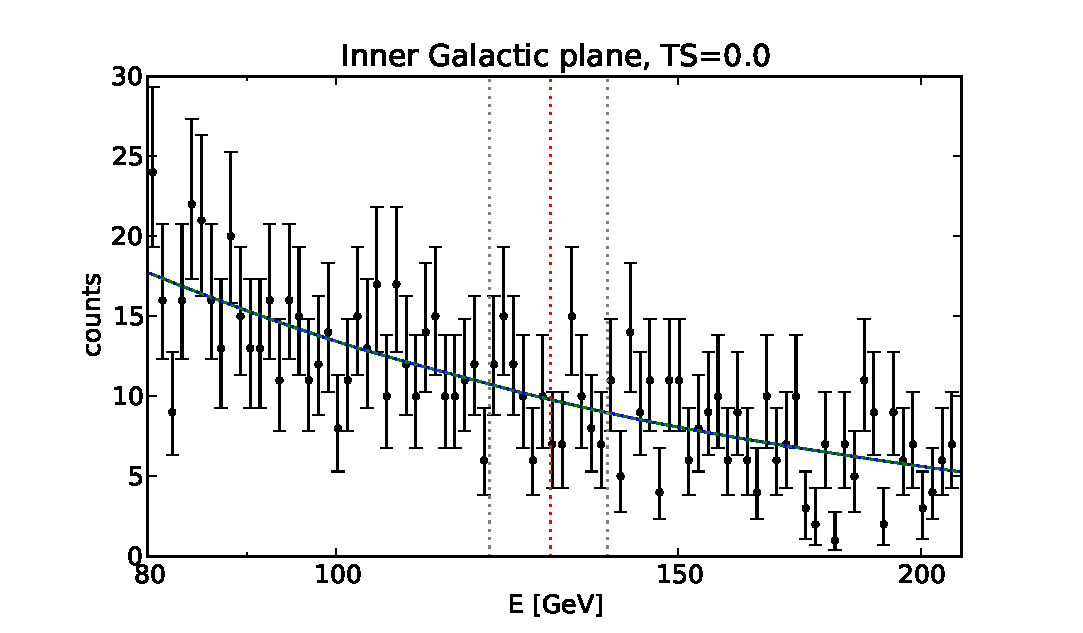
\includegraphics[width=0.48\linewidth]{plots/counts_IGP.eps}
  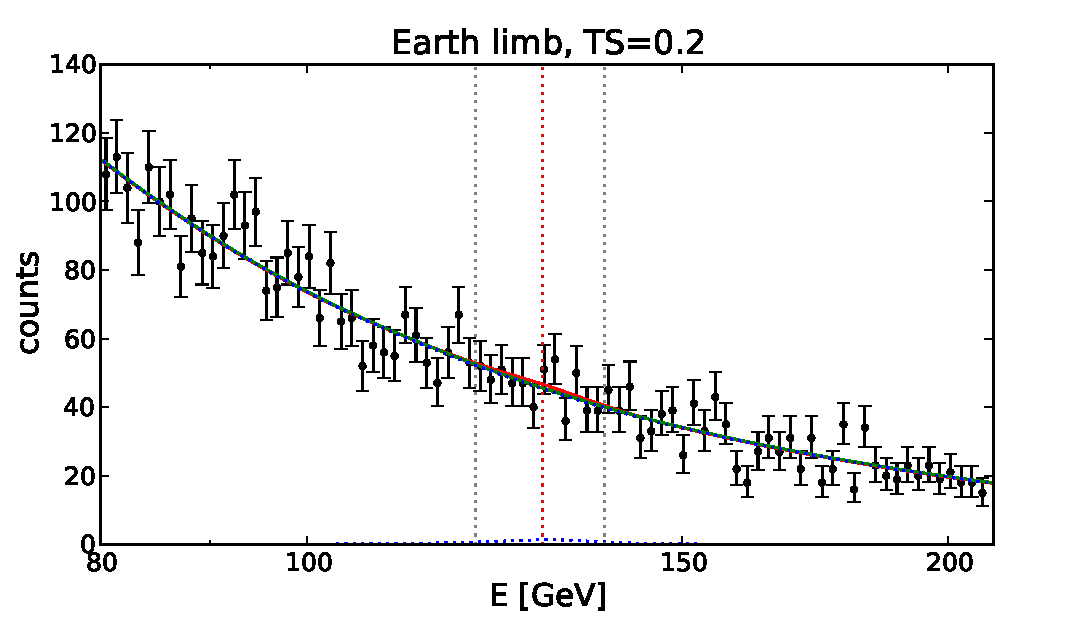
\includegraphics[width=0.48\linewidth]{plots/counts_limb.eps}
  \caption{Fits to different sets of events. The green line
  shows the null model (a power-law), whereas the red line
  shows the alternative power-law + line fit; the dotted
  blue lines are the two components of the alternative
  model. The red (black) dotted lines indicate 129 GeV
  (13.6\% FWHM around 129 GeV).}
  \label{fig:spectra1}
\end{figure*}

\begin{figure}
  \centering
  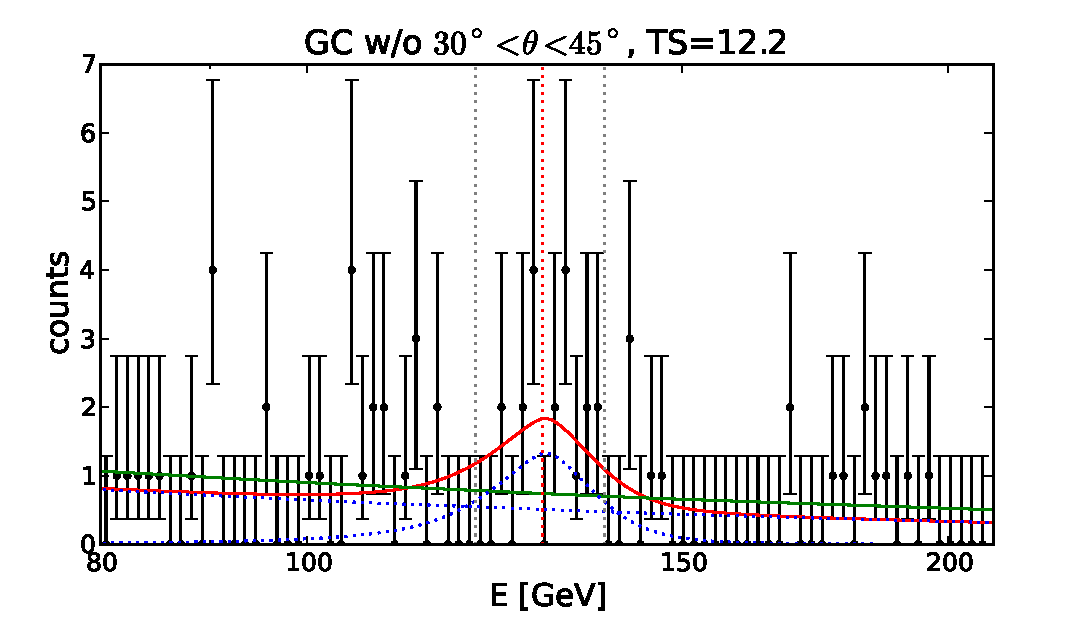
\includegraphics[width=1.\linewidth]{plots/counts_GC_wo3045.eps}
  \caption{Same as Fig.~\ref{fig:spectra1}, but for GC
  events \emph{excluding} the suspicious
  $30^\circ<\theta<45^\circ$ range.}
  \label{fig:spectra2}
\end{figure}

In Fig.~\ref{fig:spectra1} we show fits to the energy
spectra measured in different regions. The fits are
performed as in~\cite{Weniger:2012}. The $TS$ value is as
usual defined as $TS=-2\ln \mathcal{L}_{\rm
null}/\mathcal{L}_{\rm alt}$, where $\mathcal{L}_{\rm
null(alt)}$ is the likelihood of a fit without(with) line;
note that the line normalization is constrained to be
non-negative. Whereas the TS value in the GC region is in
our case with $TS=16.9$ relatively large, there is no
indication for line contributions in the Inner Galactic
plane or the full set of Earth limb photons (upper left and
lower panels of Fig.~\ref{fig:spectra1}; a suspicious subset
of limb events will be discussed below).

\emph{We emphasize that signal significances calculated from the GC region as
adopted in this paper are not sufficient to represent the full significance of
the putative signal, which is usually higher when adopting regions with
optimized signal-to-noise ratio~\cite{Weniger:2012} or a template
analysis~\cite{linepaper}. We use the GC region here since it should be
dominated by line events, making it a good starting point to look for
suspicious trends in the data.}


% CHECK: Time correlation with solar flares?

\begin{figure*}
  \centering
  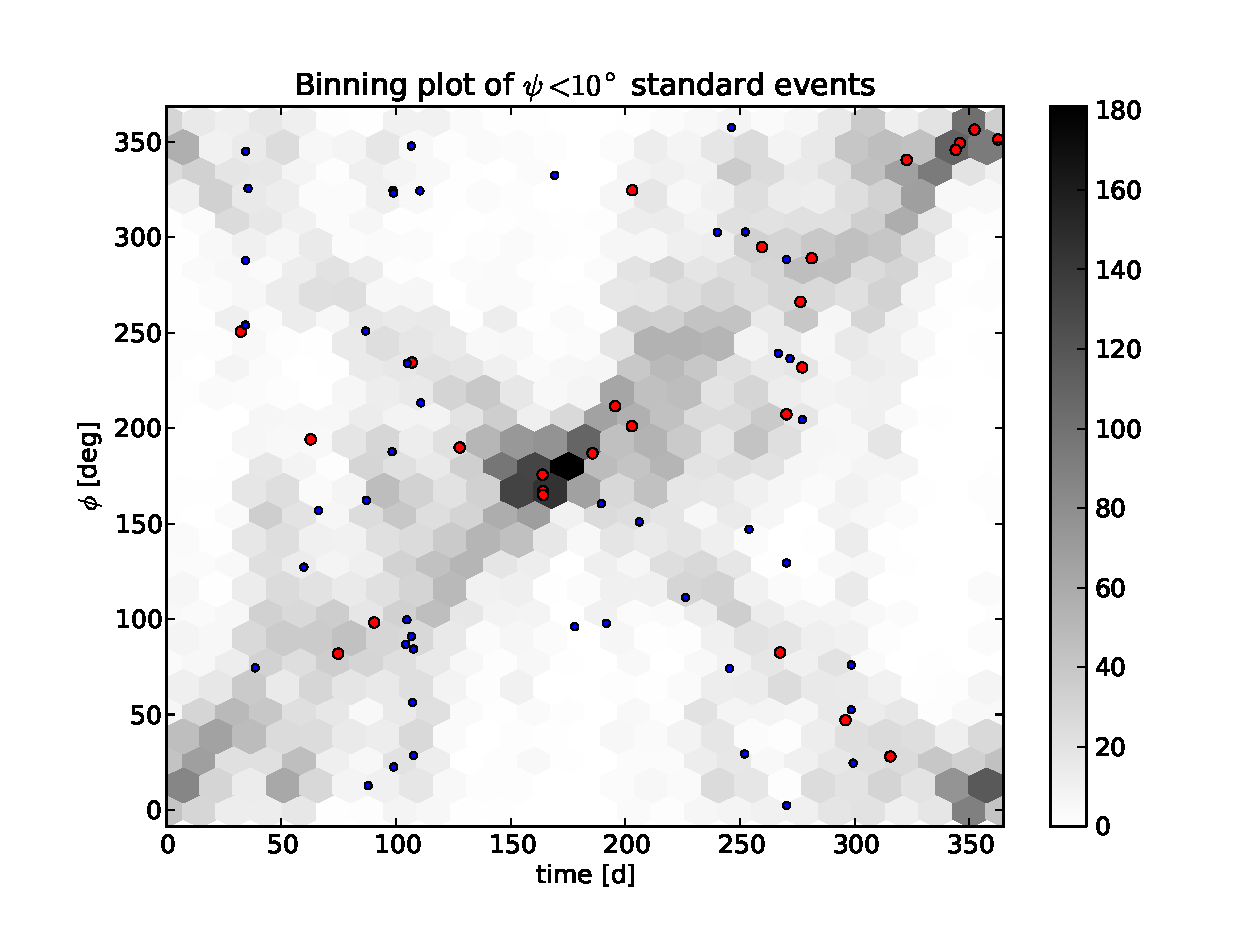
\includegraphics[width=0.44\textwidth]{plots/TIME_PHI.eps}
  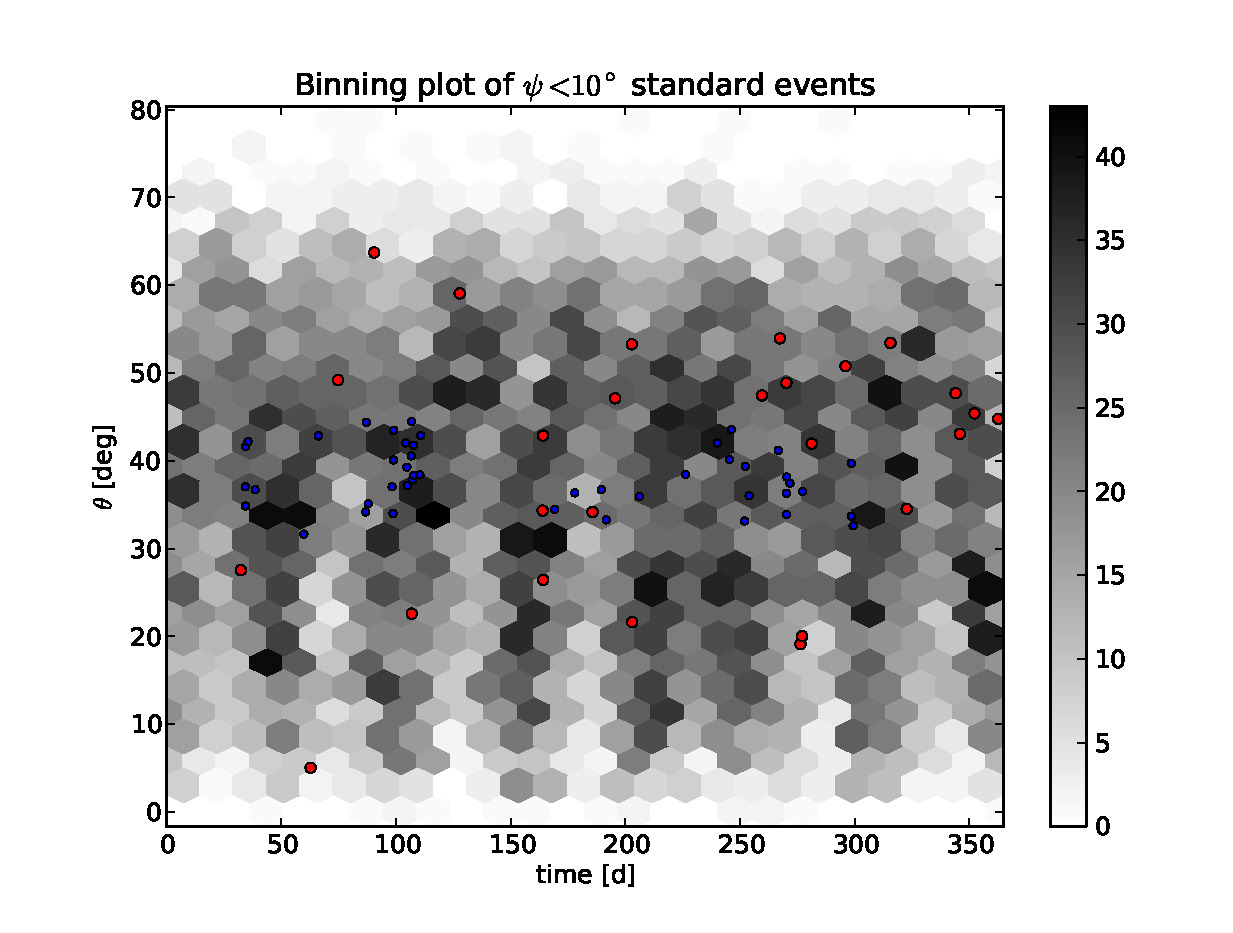
\includegraphics[width=0.44\textwidth]{plots/TIME_THETA.eps}
  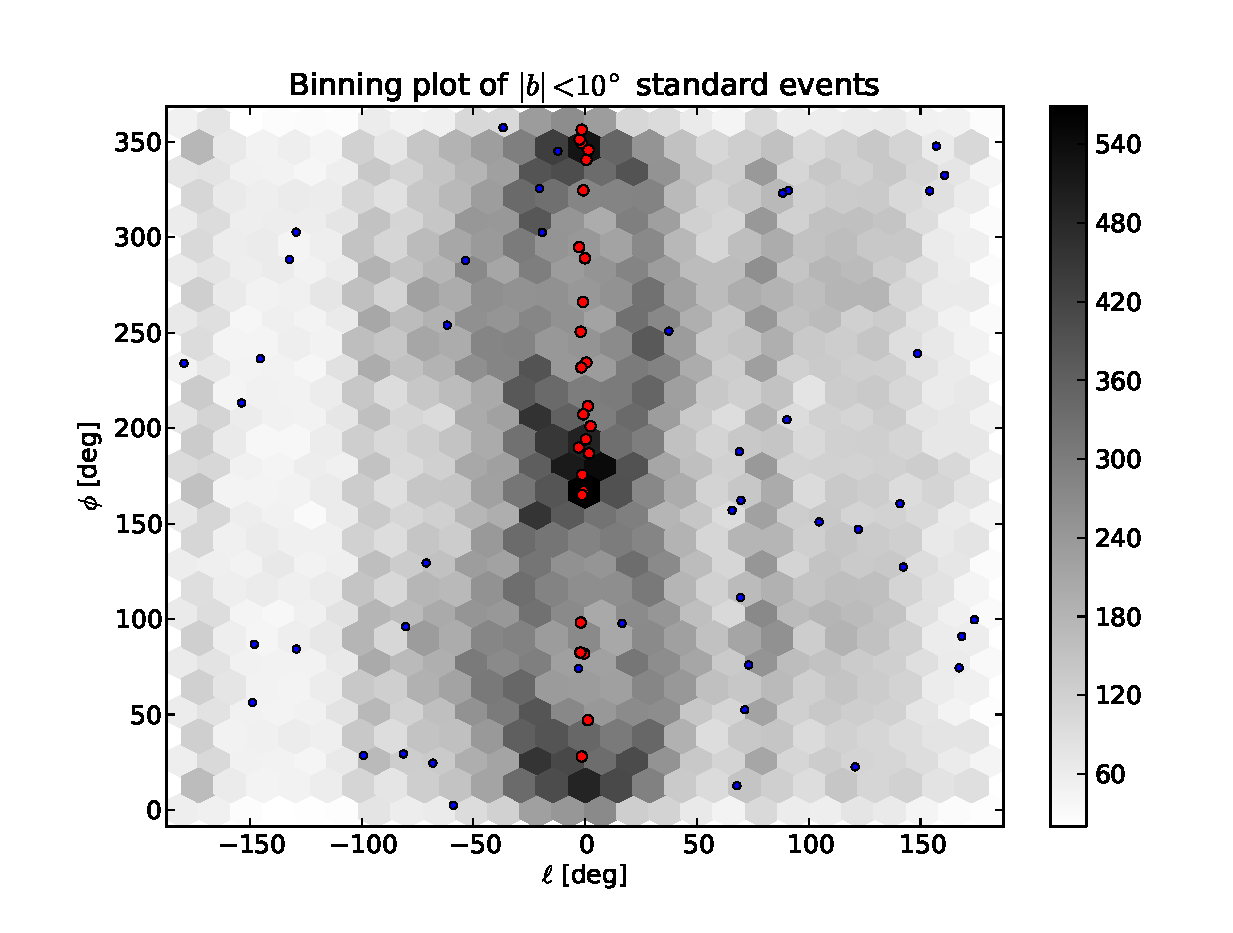
\includegraphics[width=0.44\textwidth]{plots/L_PHI.eps}
  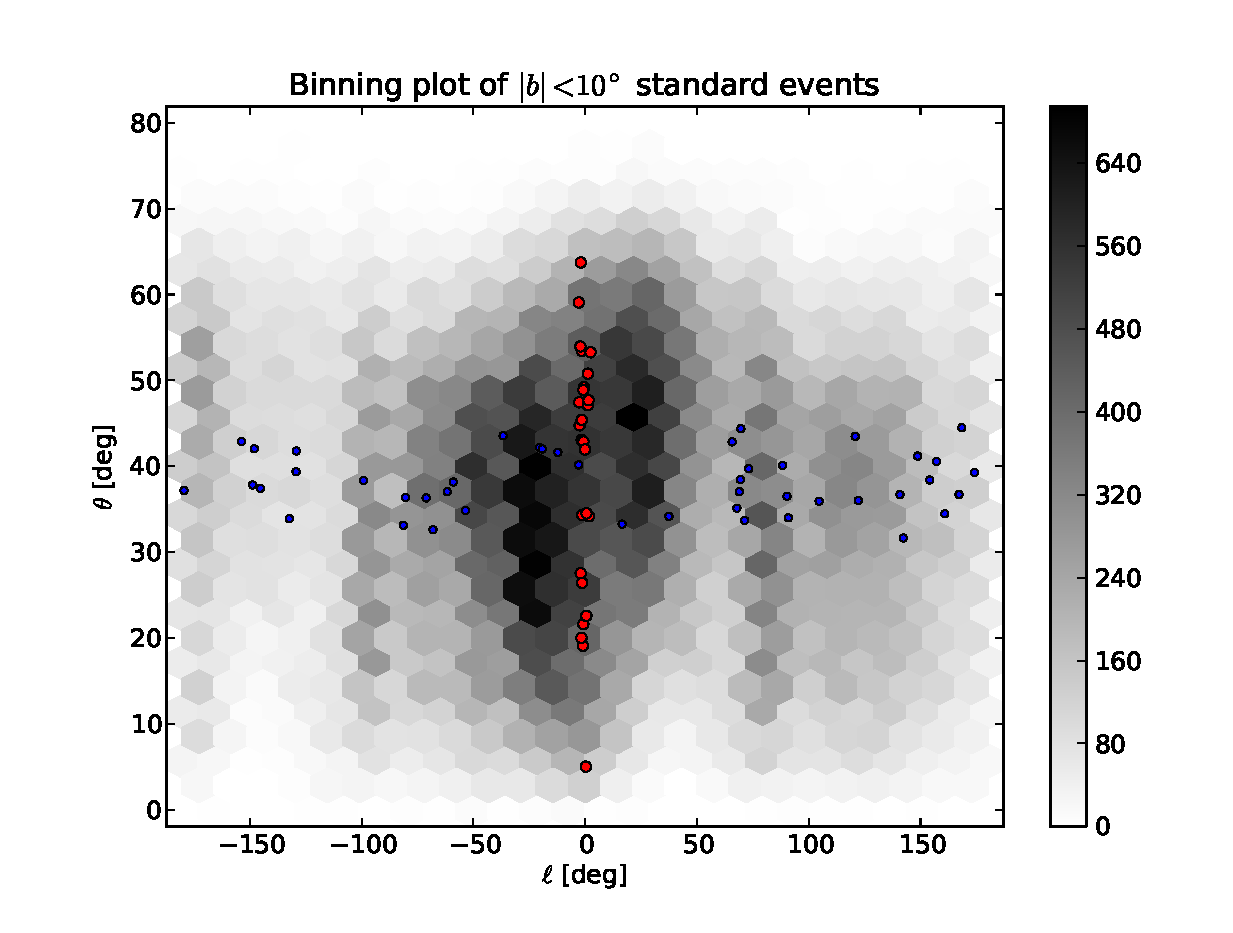
\includegraphics[width=0.44\textwidth]{plots/L_THETA.eps}
  \caption{\emph{Upper panels:} $\phi$ (left panel) and
  $\theta$ (right panel) distribution of of standard events
  close to the Galactic center, as function of time modulo
  one year (with Jan 1st at the origin). In Dec (Jun) the
  Sun passes near the Galactic center (anti-center).  In
  these periods, most events are observed at $\phi\approx
  0^\circ$ ($\phi\approx 180^\circ$), since the LAT $x-z$
  plane is determined by the Sun to keep the solar panels
  oriented. \emph{Lower panels:} $\phi$ (left panel) and
  $\theta$ (right panel) distribution of standard events
  along the galactic disk. Close to the GC, the distribution
  becomes significantly bimodal. The red and blue dots are
  as in Fig.~\ref{fig:phiThetaDist}.}
  \label{fig:time_phi}
\end{figure*}

\begin{figure}
  \centering
  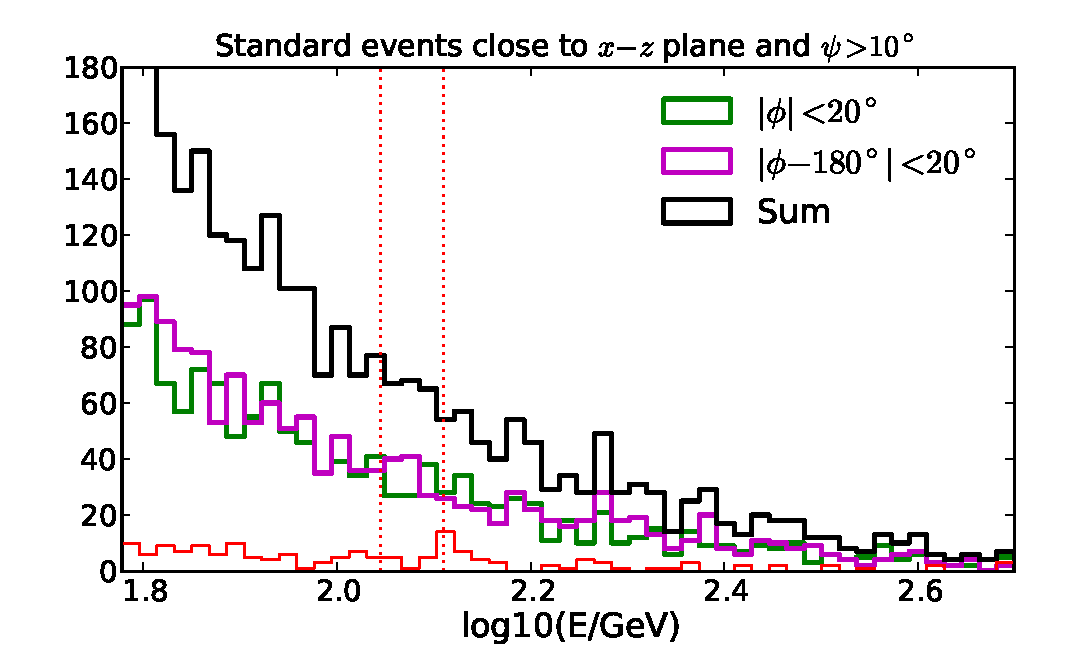
\includegraphics[width=1.0\linewidth]{plots/phi_energy.eps}
  \caption{Energy distribution of standard events away from the GC with
  incidence angles close to the LAT $x-z$ plane (perpendicular to the solar
  panels). The red dotted lines indicate 111 and 129 GeV; the thin red line
  shows GC events for comparison.}
  \label{fig:spectrum_phi}
\end{figure}

\subsubsection{Hypothesis: The spectra at the Galactic
center are hard, making energy mapping errors more
significant}

The Galactic center might harbour an unusually large number
of sources with very hard spectra. If these high energy
photons are occasionally mis-reconstructed with energies
close to 130 GeV, this could produce a line feature in the
data that would dominantly show up at the Galactic center.
In Tab.~\ref{tab:regions}, we list the ratio of $>300\GeV$
events to $>100\GeV$ events and of $>100\GeV$ to $>30\GeV$
events, in different regions of the sky.  Interestingly, the
Galactic center does not harbour significantly more high
energy events than other regions of the sky with higher
statistics but no feature at 130 GeV (see above). Note that
about $\sim15$ events contribute to the central part of the
line feature seen at the GC. Assuming that fluxes are not
harder than $dN/dE \propto E^{-2.0}$ (normalized to the
number of events above 150 GeV), the GC events cannot come
from energies above 300 GeV, since there would be not enough
events to make up the 130 GeV excess even if \emph{all} of
them were incorrectly mapped to 130 GeV. 

\subsubsection{Hypothesis: the GC observations have a
restricted range of incidence angles on the instrument}

In case the Galactic center is predominantly observed under
specific angles in LAT instrumental coordinates, associated
instrumental problems could be projected onto the Galactic
center simply for geometrical reasons. The sky coverage of
Fermi at various incidence angles is usually approximately
uniform, but this is not necessarily the case for the
Galactic center.  In late December (June), the angular
distance between the Sun and the Galactic center
(anti-center) reduces to about $5^\circ$.  Since Fermi keeps
the solar panels aligned to the Sun, this leads to an
increase of Galactic center events at instrument azimuth
angles of $\phi\approx 0^\circ$ ($\phi\approx 180^\circ$).
This behaviour is clearly visible in the upper left panel of
Fig.~\ref{fig:time_phi}, where we show the $\phi$
distribution of $>10\GeV$ events from the Galactic center as
a function of time (modulo one year).  The $\theta$
distribution in the upper right panel reflects the
precession pattern with a $\sim55$ day period. Integrated
over time, the $\phi$ and $\theta$ distributions look like
in the lower panels of Fig.~\ref{fig:time_phi}.

It is tempting to relate the locality of the 130 GeV excess
in the Galactic plane to this inhomogeneous $\phi$
distribution. As a test, we select standard events from the
full sky (excluding $\psi < 10^\circ$) in the range $\phi=
-20\dots20^\circ\ \text{mod}\ 180^\circ$. The total number
of these events is $\sim10$ times larger than the number of
Galactic center events; an anomaly in the event
reconstruction under these $\phi$ angles should appear in
this data sample with high significance.  However, the
energy distribution shown in Fig.~\ref{fig:spectrum_phi}
shows no significant feature at 111 or 130 GeV.

\begin{figure*}
  \centering
  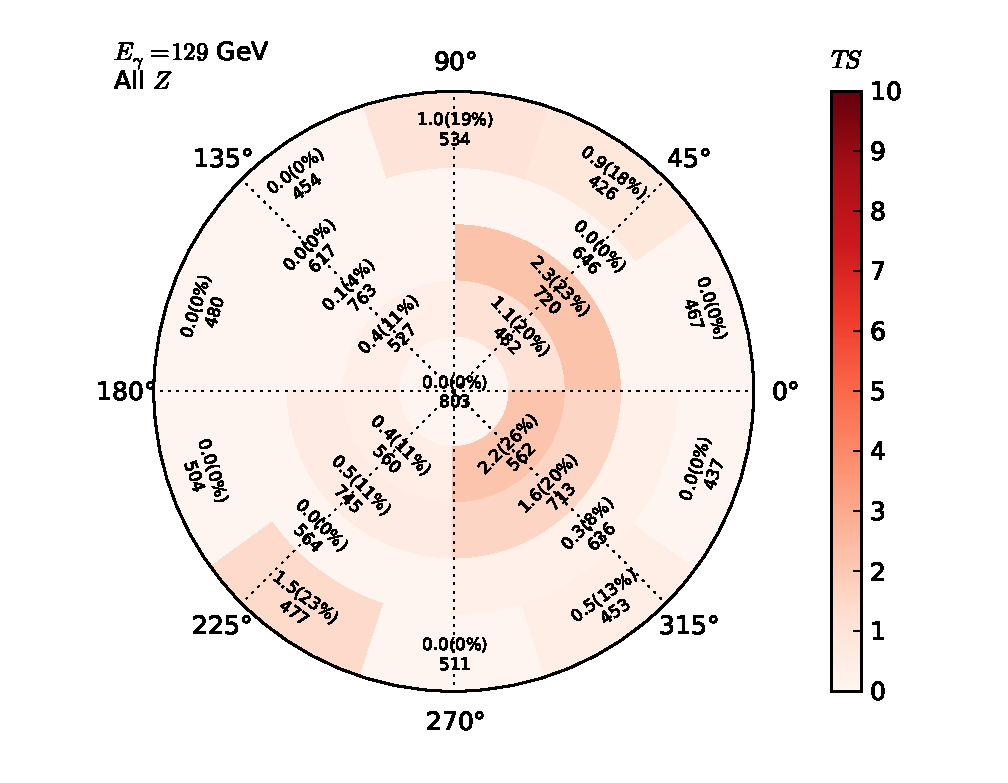
\includegraphics[width=0.45\textwidth]{plots/polar_all.eps}
  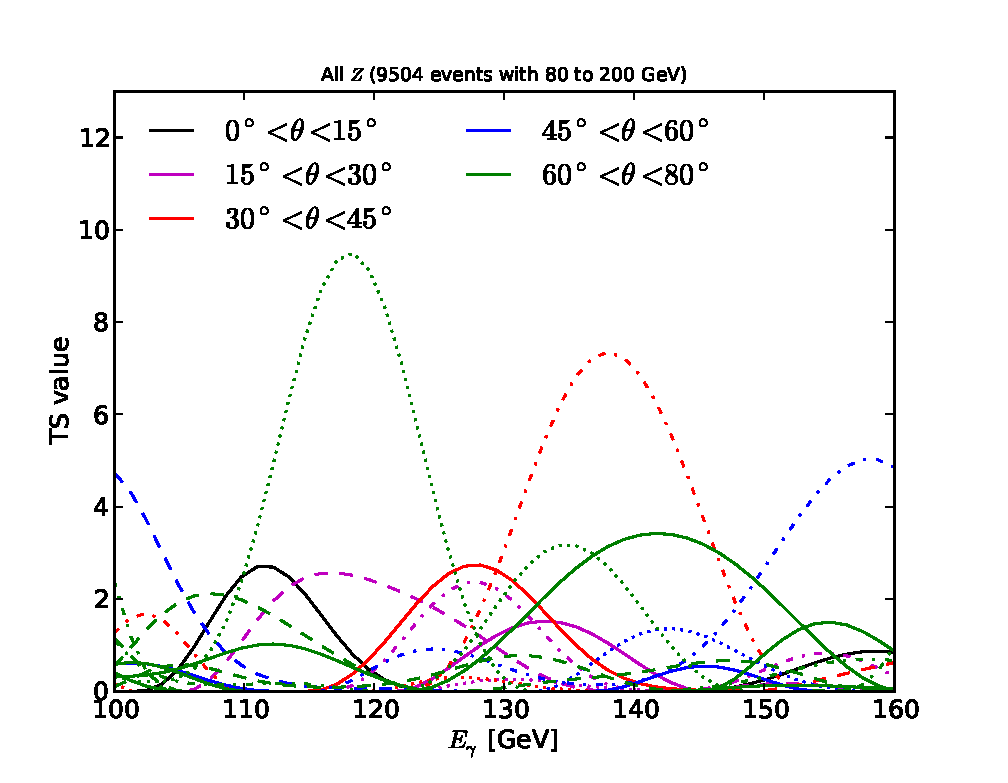
\includegraphics[width=0.40\textwidth]{plots/scan_all.eps}
  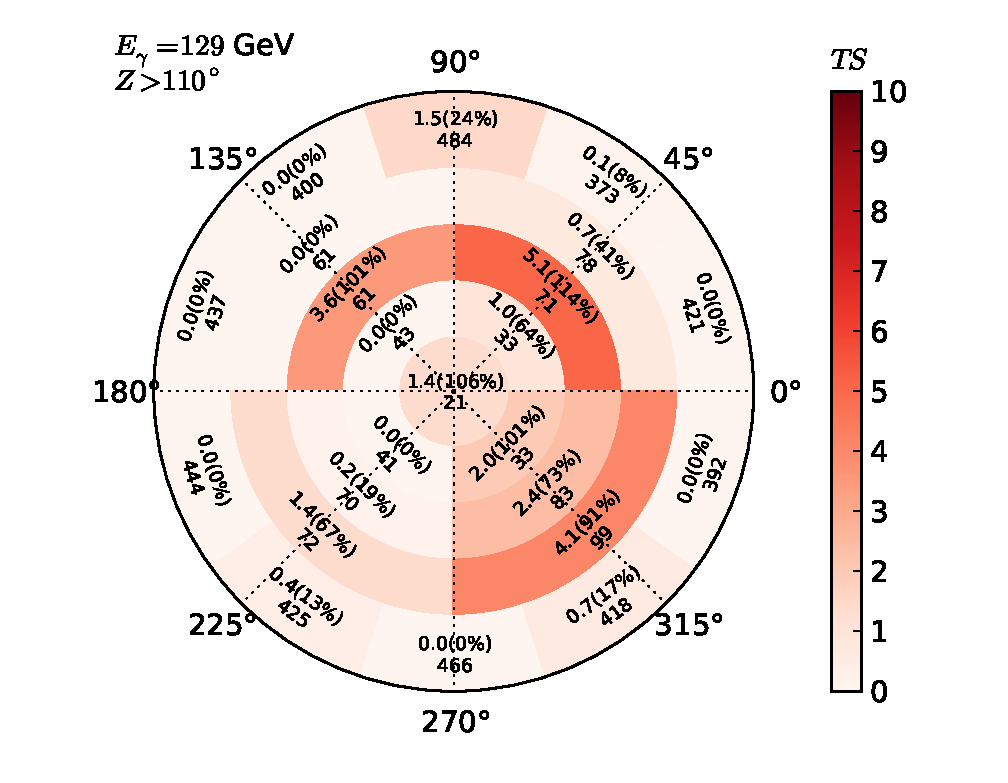
\includegraphics[width=0.45\textwidth]{plots/polar_z.GT.110.eps}
  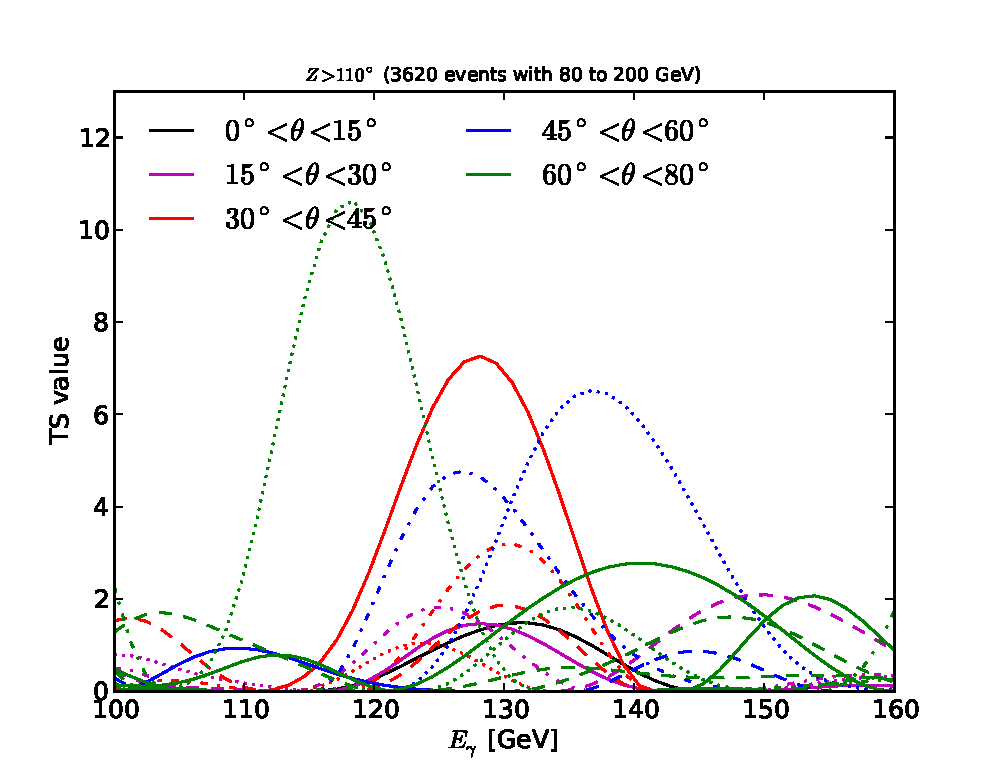
\includegraphics[width=0.40\textwidth]{plots/scan_z.GT.110.eps}
  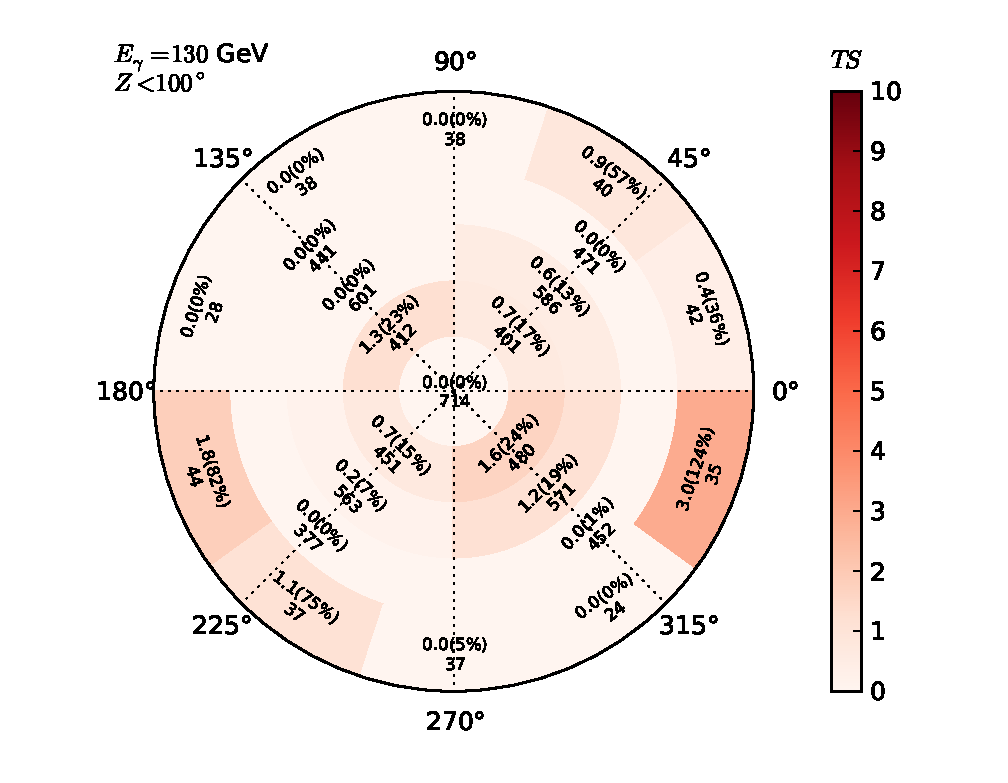
\includegraphics[width=0.45\textwidth]{plots/polar_z.LE.100.eps}
  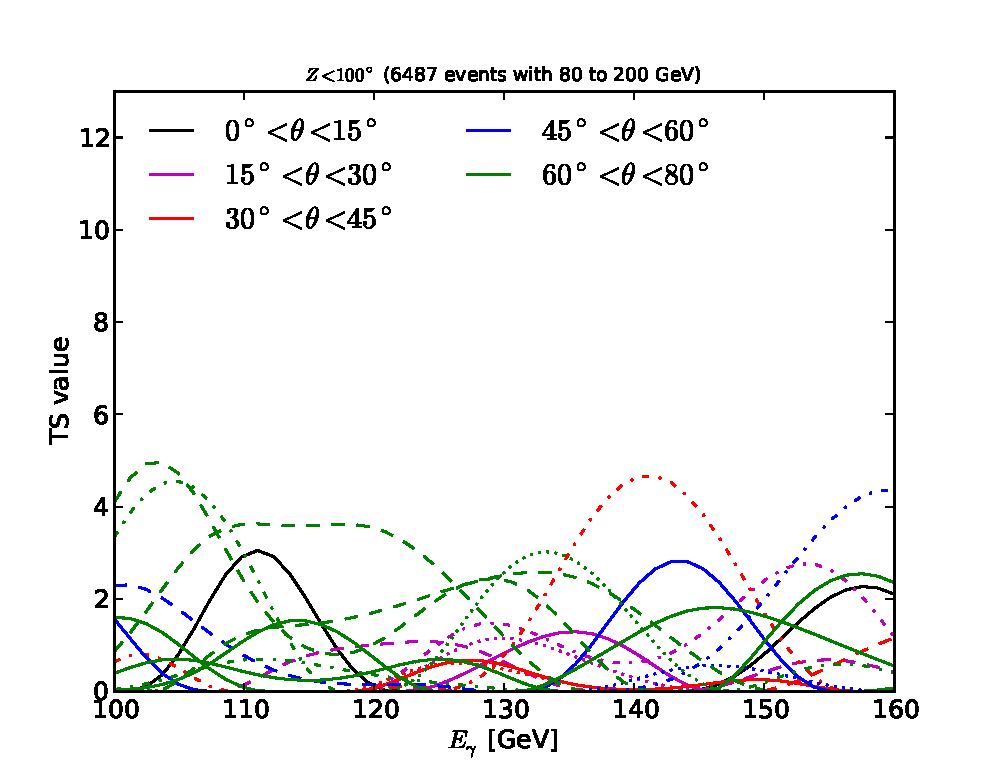
\includegraphics[width=0.40\textwidth]{plots/scan_z.LE.100.eps}
  \caption{\emph{Left panels:} Significance for a 130 GeV
  line-like excess in different parts of the $\theta$-$\phi$
  plane (for $\theta=0$--$80^\circ$). From top to bottom,
  the results are derived from all events, from the Earth
  limb events, and from standard events. The three numbers
  show the TS value for the presence of a 130 GeV line, the
  signal-to-background ratio and the number of events above
  $80\GeV$ inside the considered $\theta$-$\phi$ region.
  \emph{Right panels:} The significance for a $E_\gamma$
  line-like excess for the same $\theta$-$\phi$ regions.}
  \label{fig:polarPlotsAll}
\end{figure*}


\subsection{Peculiarities of the instrument}
Instrumental effects are likely to be correlated with
specific instrumental coordinates rather than sky
coordinates. In this subsection we will search for
suspicious trends at 130 GeV as function of the event
incidence angles, event quality parameters, the time
evolution of the GC signal, and check for the possibility of
`hotspots' at other regions of the sky.

\subsubsection{Hypothesis: A 130 GeV features is visible
under specific incidence angles on the instrument}

% Intro

An interesting concern is that a 130 GeV feature in the
reconstructed events is visible only for events with certain
incidence angles $(\theta, \phi$) in instrumental
coordinates. The 130 GeV excess would be then imprinted on
regions of the sky that are predominantly observed under
these problematic angles. A study in terms of instrumental
$x-y-z$ coordinates is not possible using public data only.
It is however difficult to conceive how these conditional
parameters could be correlated with certain regions of the
sky.

To study line-like features under different incidence
angles, we split up the $(\theta, \phi)$ plane in different
regions as shown in the left panels of
Fig.~\ref{fig:polarPlotsAll}. We then analyse the spectrum
of all events that hit the detector under these incidence
angle patches separately and search for lines. The fits are
performed as in Ref.~\cite{Weniger:2012}, but the energy
window is fixed to 80 to 200 GeV, we assume a flat
acceptance and as line we take a simple Gaussian with $6\%$
width.

The left panels of Fig.~\ref{fig:polarPlotsAll} show from
top to bottom the results obtained (1) using all events, (2)
using Earth limb events only, and (3) using standard events
only; the latter two are obviously disjunct subsets of the
former one. For each $(\theta, \phi)$ range we quote three
numbers: the significance of a 130 GeV line-feature in terms
of the $TS$ value, the signal-to-background ratio of the
putative line signal, and the number of events above 80 GeV
that contribute to this region. The $TS$ values are also
shown by the colors for better visibility.

% Indication for correlation with $Z$ angle or statistical
% fluke
% GC line only for 50 rocking angles
% GC line independent of this range

As a further check whether energies around 130 GeV are in
some unexpected way distinct, we search for line-like
features at other energies from 100 to 160 GeV. The
resulting $TS$ values as function of the line energy are
shown in the right plots of Fig.~\ref{fig:polarPlotsAll}. In
particular the lower two plots which correspond to
independent data sets show clearly that the enhanced $TS$
values at different energies in different panels are not
correlated. Lastly, we note that the significance of the
largest $TS$ value, $TS=10.5$, has a large $p$-value of
about $0.38$ when taking into into account
$2\times23\times2$ trials over a $\chi_{k=2}^2$ distribution
(two $Z$ ranges, $23$ incidence angle panels, $\sim2$
``independent search regions''~\cite{Vittels}).

% Move up this part
However, it cannot be entirely excluded that the energy
reconstruction under different incident angles somehow
depends on the zenith angle $Z$ of the events (e.g. if there
is a subtle dependence on the rocking angle), and that the
large $TS$ values around $\theta\sim40^\circ$ actually
indicate an instrumental effect. We will further contemplate
on this in section~\ref{sec:EarthLimb}; in any case more
Earth limb data will help to sort out this possibility.

\subsubsection{Hypothesis: The Galactic center events are flagged as badly
reconstructed}

\begin{figure}
  \centering
  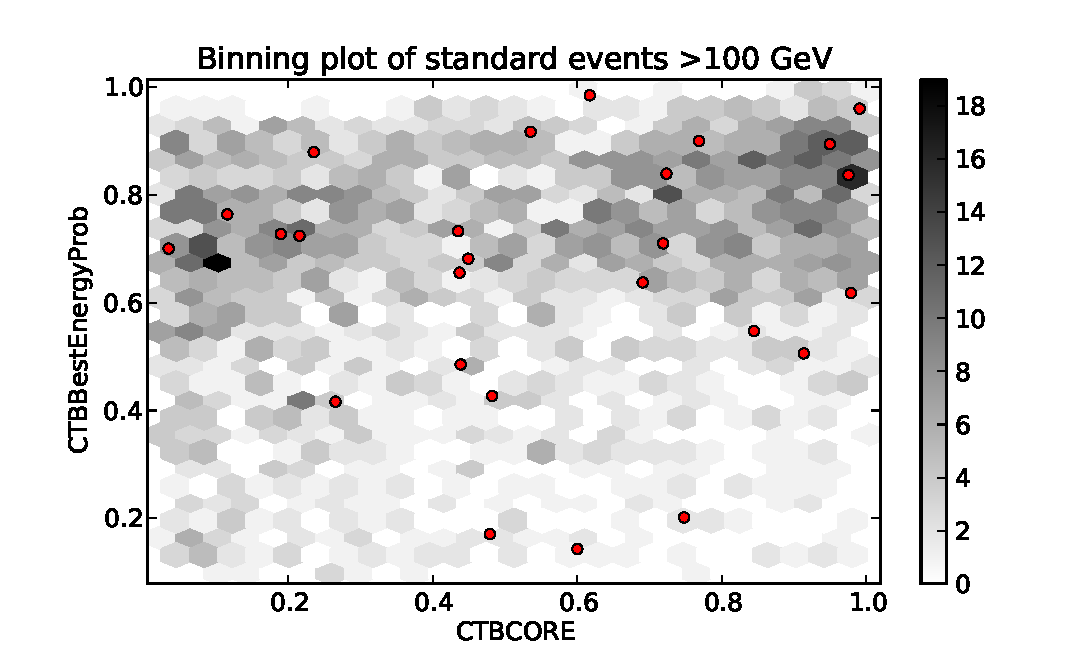
\includegraphics[width=1.00\linewidth]{plots/CTBCORE_CTBBestEnergyProb.eps}
  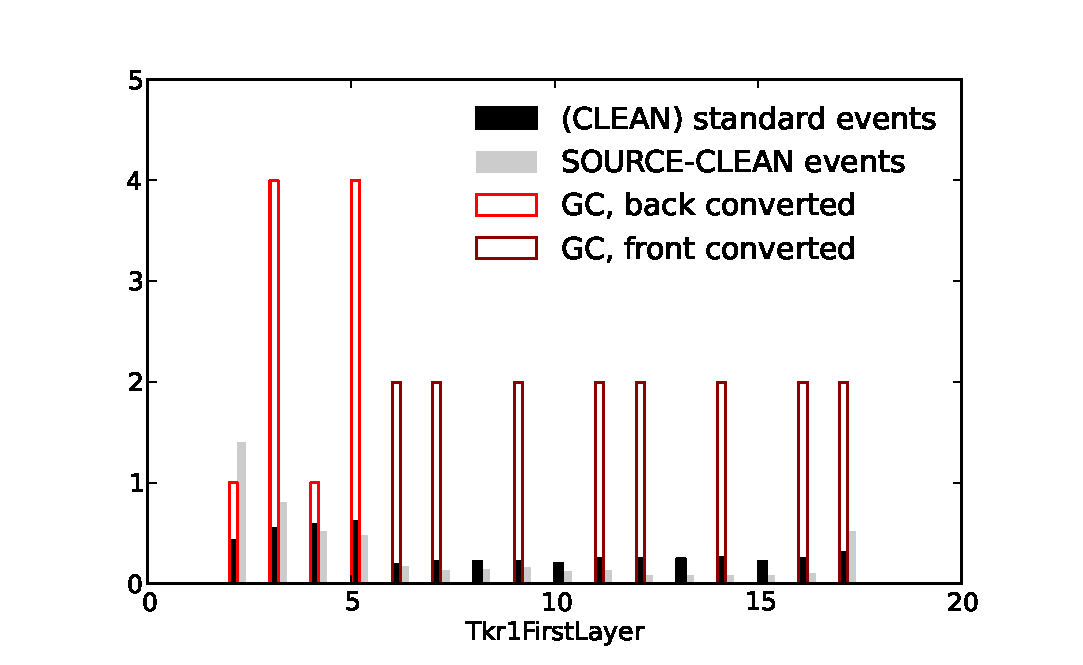
\includegraphics[width=1.00\linewidth]{plots/Tkr1FirstLayer.eps}
  \caption{\emph{Upper panel:} Distribution of CTBCORE (the
  probability that the direction estimate is good) and
  CTBBestEnergyProb (the probability that the best energy
  chosen from the two energy estimators is correct) for
  Galactic center line events (in red), compared to the
  distribution of $>50$ GeV standard events.  \emph{Lower
  panel}: First tracker layer to show evidence of a particle
  hit for the best track reconstruction. Tracker layers are
  0-17 where 0 is closest to the calorimeter, and 6-17 (2-5)
  corresponds to front- (back-)converting events (tracker
  layers 0 and 1 come without conversion foils). The gray
  bars show the distribution averaged over all $>100$ GeV
  standard events, the green/red bars show the distribution
  for the GC line.}
  \label{fig:CTBquality}
\end{figure}

The extended LAT event files contain additional information
about the quality of the event
reconstruction.\footnote{\url{http://fermi.gsfc.nasa.gov/ssc/%
data/analysis/documentation/Cicerone/Cicerone\_Data/LAT\_Data\_Columns.html}}
CTBCORE describes the probablity that the direction estimate
is good (roughly the probability that the reconstructed
direction falls within the nominal 68\% containment angle),
CTBBestEnergyProb the probability that the reconstructed
energy falls into the core of the energy dispersion. We show
these parameters for the the GC line events in the left
panel of Fig.~\ref{fig:CTBquality}; the background histogram
shows the distribuion of the these parameters in standard
events above 50 GeV. No significant bias in the distribution
is visible.

The green and red bars in the right panel of
Fig.~\ref{fig:CTBquality} show the first tracker layer that
shows evidence of a particle hit for the best track
reconstruction (Tkr1FirstLayer) in case of the GC line
events.  Tracker layers are 0--17, where 0 is closest to the
calorimeter and 6--17 (2--5) corresponds to front-
(back-)converting events (tracker layers 0 and 1 come
without conversion foils). The gray bars show the
distribution averaged over all $>100$ GeV standard events
for comparison. The distribution of GC line events is
compatible with the expectations.

\subsubsection{Hypothesis: There are `hotspots' with
line-like features in other sky regions}

\begin{figure}
  \begin{center}
    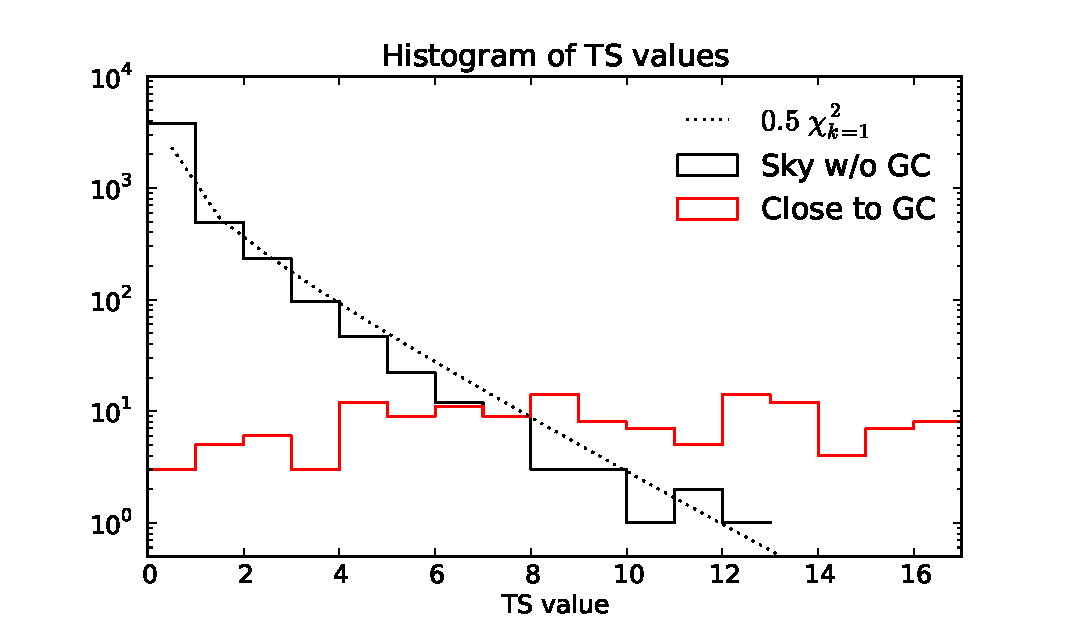
\includegraphics[width=1.0\linewidth]{plots/hotspot_histogram.eps}
  \end{center}
  \caption{Histogram of TS values observed close to the GC
  (red) and in the rest of the sky (black), compared to the
  expected distribution (dashed).}
  \label{fig:hotspots}
\end{figure}

The 130 GeV excess is located in a narrow range of about
$\sim5^\circ$ around the Galactic center. If other
significant `hotspots' (localized regions with a significant
line-like emission) would exist in the sky, this could
indicate a instrumental effect, or point to a source class
that is concentrated to the GC. In absence of knowledge
about the distribution of such a source, we adopt the
following strategy: For each standard event above 80 GeV, we
select the 103 nearest neighbour events (in physical
coordinates; 103 is the number of events in the GC region
above 80 GeV), and calculate the TS value for a line at 130
GeV. The details of the fit correspond to what we did for
e.g.~Fig.~\ref{fig:spectra1}. We exclude cases where the
nearest neighbours are closer than $10^\circ$ to the GC to
avoid contamination with the GC signature. The distribution
of TS values obtained in this way is shown in
Fig.~\ref{fig:hotspots} by the black line. Though we indeed
find places in the sky with TS values as large as $TS=13$
(which indicates a local $>3\sigma$ significance), this is
in perfect agreement with the statistical expectations as
shown by the dashed line. On the other hand, the TS value
distribution in cases where the nearest neighbours overlap
with $\ell=b=0^\circ$ shows strong deviations from the
expected distribution, as shown by the red line in
Fig.~\ref{fig:hotspots}.

\subsubsection{Hypothesis: The observed signal is variable}

\begin{figure}
  \begin{center}
    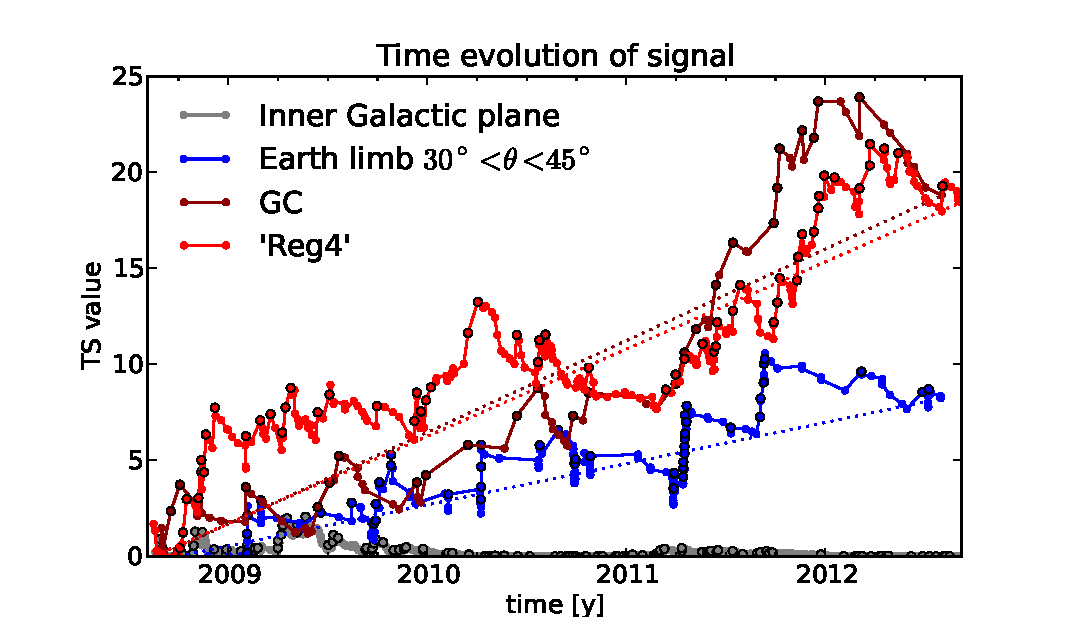
\includegraphics[width=1.0\linewidth]{plots/TS_time.eps}
  \end{center}
  \caption{Time evolution of TS values. In red we show the
  GC line, in blue the Earth limb line. Gray lines indicate
  the $68\%$ and $95\%$ CL bands for the time evolution
  obtained by removing random parts of the GC events as seen
  today.}
  \label{fig:timeevolution}
\end{figure}

The most common interpretations of the 130 GeV excess (in
terms of dark matter annihilation) would predict a steady
source. On the other hand, a strong variability could
indicate time-dependent instrumental effects. In
Fig.~\ref{fig:timeevolution} we plot how the $TS$ value of
the signal in the GC region evolved over time (red);
compared to the time-evolution of the suspicious Earth limb
line (blue). The GC curve appears to have grown most
strongly during March 2011 and February 2012, and falling
during last few months, but it lies mostly within the
statistical expectations for a steady source. The number of
GC line events (shown by the larger red circles in
Fig.~\ref{fig:timeevolution}) in the first and second half
of the observational period are respectively 12 and 14, and
consistent with a non-variable flux. However, a further
substantial decrease of the significance of the GC line
signal would start to challenge any dark matter related
interpretation.  In any case, the (very weak) indication for
a temporal pattern is not observed in case of the Earth limb
line. 

% \clearpage
%%%%%%%%%%%%%%%%%%%%%% SECTION III %%%%%%%%%%%%%%%%%%%%%%%%%%%%%%%
\section{Earth limb photons}
\label{sec:EarthLimb}

%%%%%%%%%%%%%%%%%%%%%%%%%%%%%%%%%%%%%%%%%%%%%%%%%
\begin{figure}
  \centering
  \includegraphics[width=1.0\linewidth]{plots/theta-E.ps}
  \caption{Incidence angle $\theta$ vs. log $E$ for $Z >
  105\degree$.  A blue box indicates the region $30\degree <
  \theta < 45\degree$ and 125 GeV $< E <$ 140 GeV, where an
  excess of events appear.  The vast majority of limb events
  are at $\theta > 60\degree$ because the telescope seldom
  points more than $50\degree$ from zenith, and the limb
  events are mostly at $Z>110\degree$.}
  \label{fig:theta-E}
\end{figure}

\begin{figure}
  \centering
  \includegraphics[width=0.45\textwidth]{plots/theta-E-frontback.ps}
  \caption{Same as \ref{fig:theta-E} but for front and back
  converting events.}
  \label{fig:theta-E-frontback}
\end{figure}


\begin{figure}
  \centering
  \includegraphics[width=1.0\linewidth]{plots/Ehist-all.ps}
  \caption{Histogram of limb $(Z>105\degree)$ events vs.
  log($E$) for various ranges of $\theta$. The position of
  the 130 GeV line is indicated (red dotted line).  Note the
  excess in the $30\degree < \theta < 45\degree$ bin, which
  contains about 5\% of the limb events.}
  \label{fig:Ehist-all}
\end{figure}

% \begin{figure*}
%   \centering
%   % 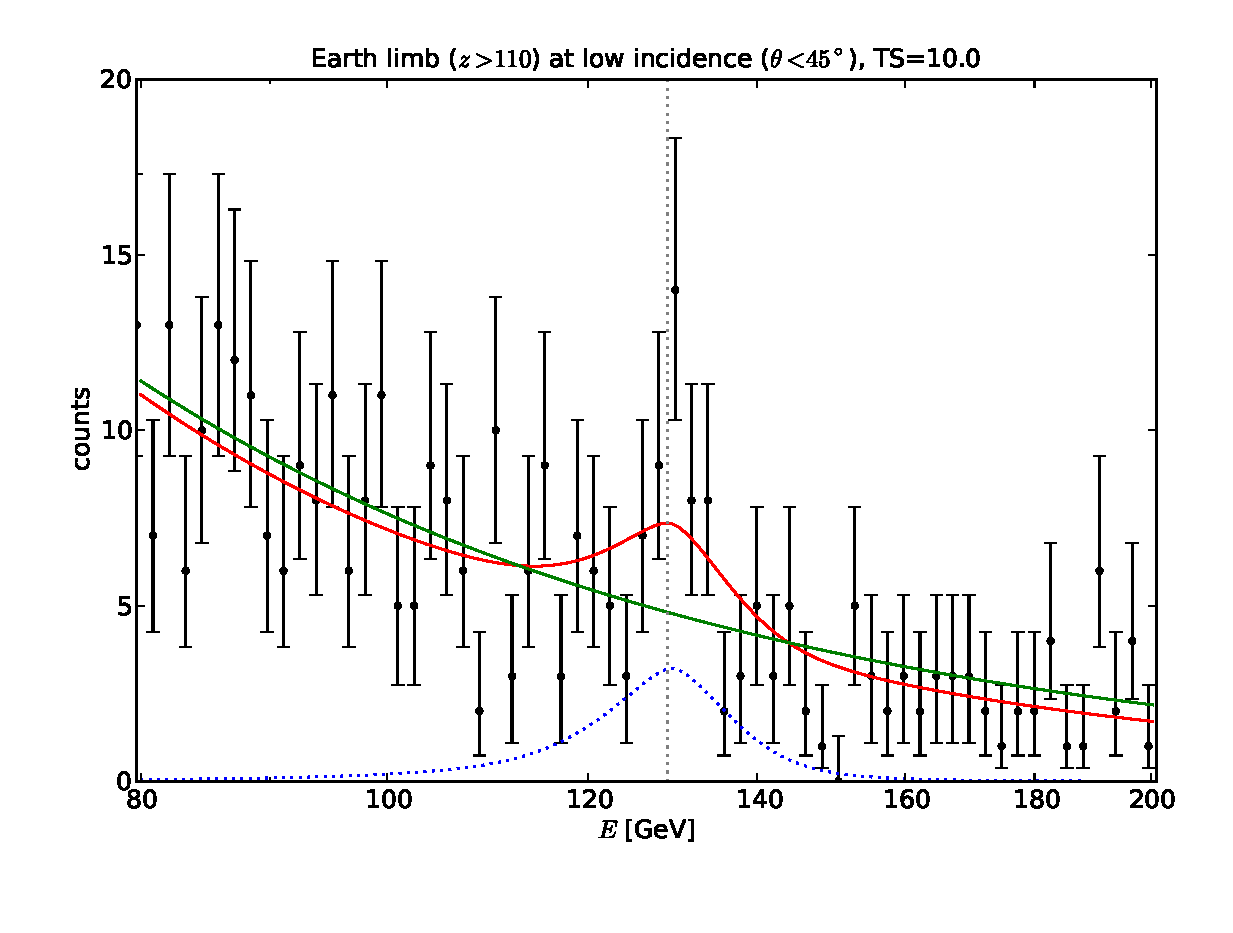
\includegraphics[width=0.48\linewidth]{plots/albedo_line_thetaCut.eps}
%   % 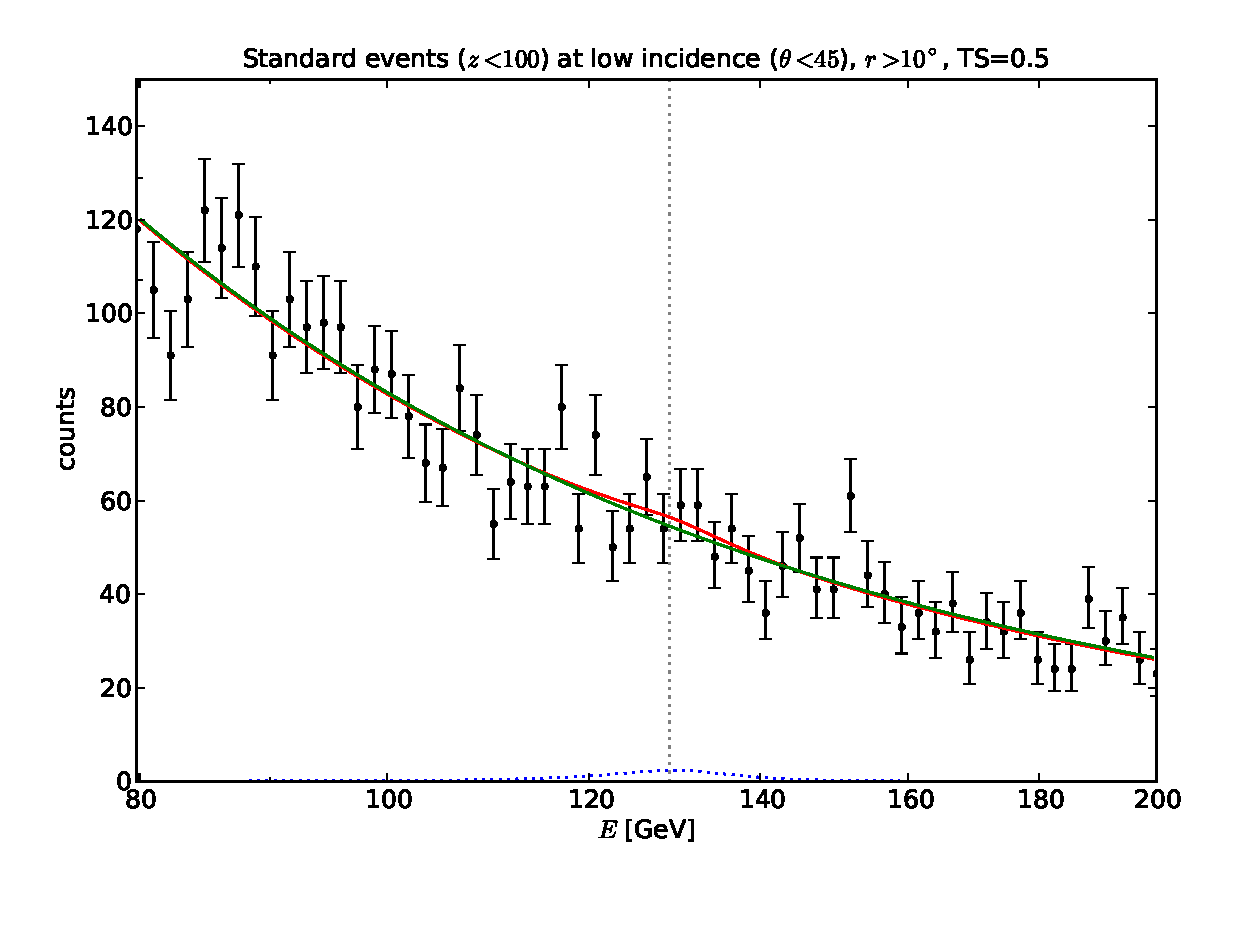
\includegraphics[width=0.48\linewidth]{plots/noalbedo_line_thetaCut.eps}
%   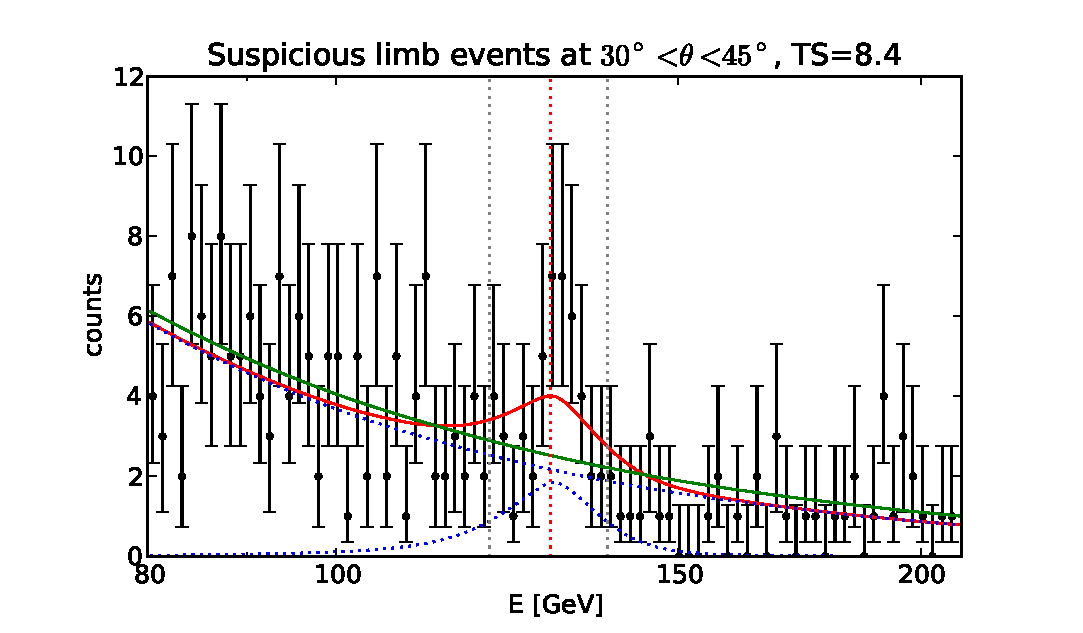
\includegraphics[width=0.48\linewidth]{plots/counts_suspiciousLimb.eps}
%   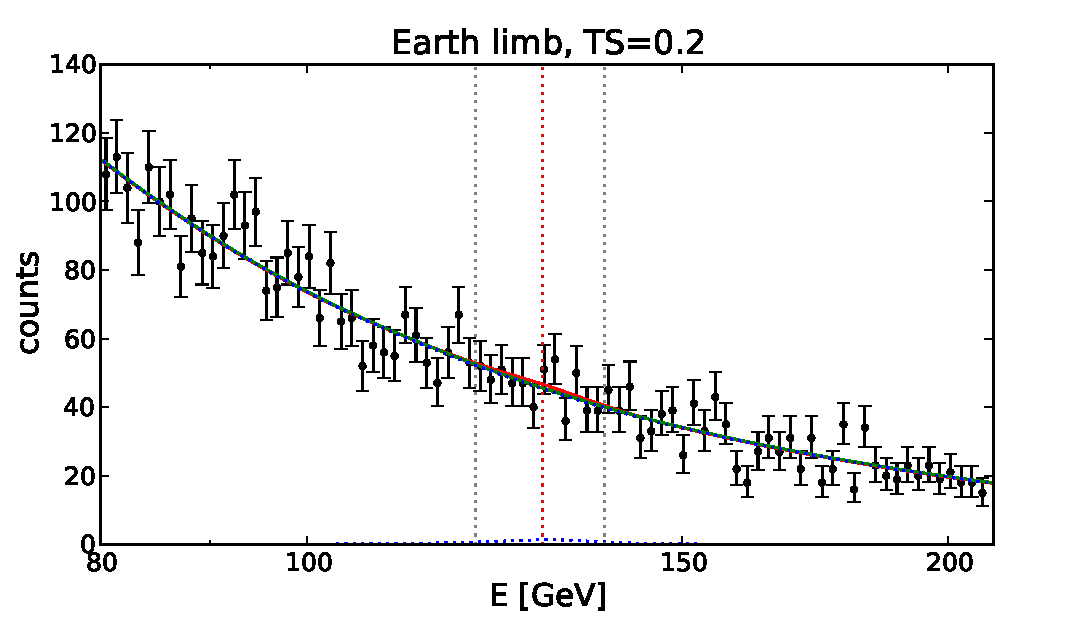
\includegraphics[width=0.48\linewidth]{plots/counts_limb.eps}
%   \caption{\emph{Left panel:} Fit of a monochromatic line at 129 GeV to the
%   low incidence angle Earth limb data. A 129 GeV line has a local significance of
%   3.2$\sigma$.  \emph{Right panel:} same, but for the low incidence angle
%   standard events. The inner $10^\circ$ around the Galactic center is masked
%   out. We find no indication for a line at 129 GeV.}
%   \label{fig:albedoline}
% \end{figure*}
% 
\begin{figure}
  \centering
  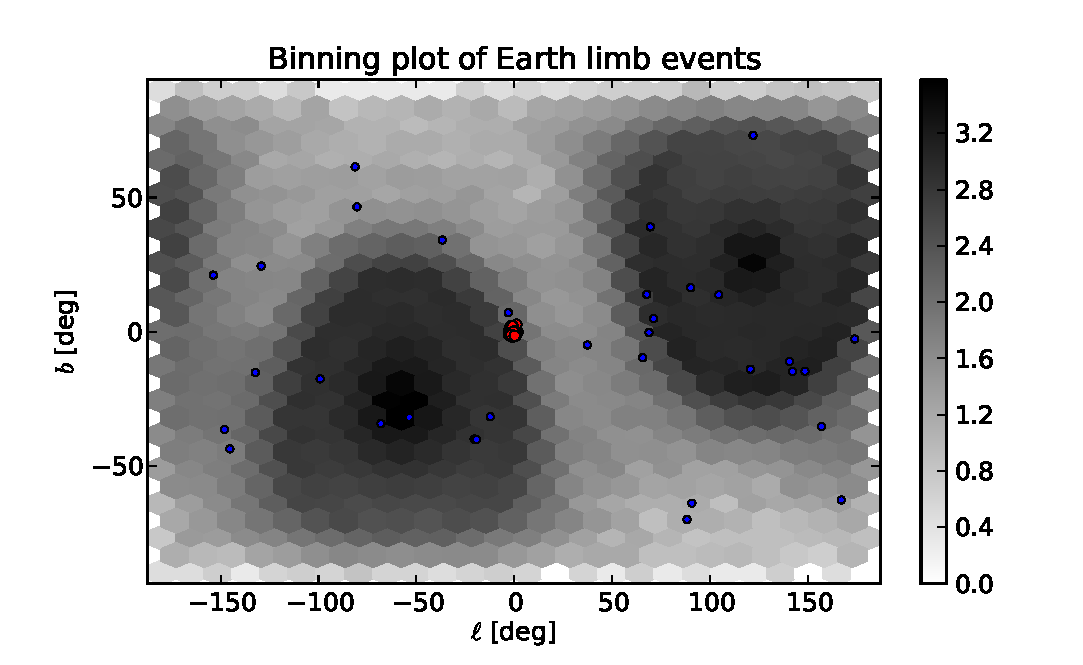
\includegraphics[width=1.0\linewidth]{plots/limb_l_b.eps}
  \caption{Same events, projected as an equal-area plot of
  Galactic $(\ell, \sin b)$.  The majority of high-incidence
  limb events appear near the orbital pole, which precesses
  around the celestial pole.  This pattern is expected from
  the observing strategy.}
  \label{fig:l-b}
\end{figure}

\begin{figure}
  \begin{center}
    % \includegraphics{<+file+>}
    \fbox{\Huge Figure}
  \end{center}
  \caption{GC and limb events. Rocking angle vs. time.}
  \label{fig:rockTime}
\end{figure}

\begin{figure}
  \centering
  \includegraphics[width=0.45\textwidth]{plots/timehist.ps}
  \caption{Time histogram (1-day bins) of suspicious limb
  events and all limb events.  The suspicious events are
  only observed at high rocking angles that occur during
  pointed observations.}
  \label{fig:timehist}
\end{figure}

\begin{figure}
  \centering
  \includegraphics[width=0.45\textwidth]{plots/Ehist-frontback.ps}
  \caption{Energy histogram as in Figure
  \ref{fig:Ehist-all}, but for front (upper panel) and back
  (lower panel) converting events. The 130 GeV excess
  appears equally in front and back converting events.}
  \label{fig:Ehist-frontback}
\end{figure}

\begin{figure}
  \centering
  \includegraphics[width=1.0\linewidth]{plots/limb_bump_model.ps}
  \caption{Upper panel: function mapping true energy $E_t$
  to reported energy $E$ (see Eqs. \ref{eq:yofx} and
  \ref{eq:dydx}).  Middle panel: The effect of this mapping
  on a spectrum of constant $dN/d\log E_t$, as in Eq.
  \ref{eq:dndy} (red line) and also for mock data (black
  histogram).  Lower panel: Same, but for $dN/dE \sim
  E^{-2.6}$.}
  \label{fig:bumpmodel}
\end{figure}

\begin{figure*}
  \centering
  \includegraphics[width=0.8\textwidth]{plots/limb_bump_model_many.ps}
  \caption{Ten mock spectra of an underlying spectrum $dN/dE
  \sim E^{-2.6}$, distorted according to Eq. \ref{eq:dndy}.
  Note the similarity to the $30\degree < \theta <
  45\degree$ panel in Figure \ref{fig:Ehist-all}.}
  \label{fig:bumpmodelmany}
\end{figure*}

\begin{figure}
  \centering
  \includegraphics[width=1.0\linewidth]{plots/limbfits.ps}
  \caption{Fits of the energy mapping model to limb data for
  various ranges of inclination angle $\theta$.  The
  vertical red dotted line corresponds to 130 GeV.  The test
  statistic ($2\Delta\ln L$) for the best fit model (green
  line) relative to the null hypothesis (red line) is given,
  along with the significance, expressed in ``sigma''
  including a penalty for the 3 additional degrees of
  freedom.  The deviation from linearity is only significant
  in the $30\degree < \theta < 45\degree$ panel, but in events with other incidence angles.}
  \label{fig:limbfits}
\end{figure}

%%%%%%%%%%%%%%%%%%%%%%%%%%%%%%%%%%%%%%

In this section we follow the weak indication of the limb
photon excess at $\sim$130 GeV and discuss the limb photons
in more detail. We show that the critical incident angles
are not (solely) responsible for the GC excess.

We begin by examining the limb events and finding a bump at
130 GeV in a subsample of these events.  We consider two
hypothesis for the origin of the bump: that the events come
from far away in energy, or the more subtle possibility that
an energy mapping error could redistribute in energy, making
a spectral feature.  We then explore the various parameters
of the GC line events and the limb bump events.  \medskip

Nearly grazing incident cosmic rays interacting with Earth
atmosphere produce cascade showers with forward-moving
gamma-rays which can penetrate the upper thin layer of
atmosphere without strong attenuation and produce a bright
gamma-ray horizon. As an Earth-orbiting gamma-ray detector,
the Earth atmosphere is the brightest source in the sky due
to its proximity to LAT. The gamma-ray emission from Earth
is produced by cosmic-ray (mostly protons, helium, and
heavier nuclei) interactions with atmosphere material. Earth
limb gamma-rays at$\sim$100 GeV are mainly from the decay of
neutral pions and kaons. At this energy, due to the
kinematics of the collisions, the cross section are peaked
in the forward direction, and the back-scattered secondary
particles at large angles relative to the direction of the
cosmic-ray cascade is very rare.

At an altitude $a$, the geometric (unrefracted) horizon is
at zenith angle \be Z_{\rm hor} =
\cos^{-1}\left(\frac{R_\oplus}{R_\oplus+a}\right)+90\degree
\ee The Fermi orbit is nearly circular with 535~km $< a <$
564~km, yielding $Z_{\rm hor}$ in the 112.7$\degree$ to
113.3$\degree$ range, with the tangent point some 2400 km
distant.  At this distance, the 90 km height of the
atmosphere subtends about $2\degree$, or roughly $111\degree
< Z < 113\degree$.

The continual cosmic-ray cascades in the Earth's atmosphere
produce gamma rays with $dN/dE \sim
E^{-2.8}$~\citep{FermiLimb}. These atmospheric gammas are
referred to as ``Earth limb photons'' or sometimes as
``albedo photons.''  These photons provide a convenient
reference sample to search for systematics in the LAT data.
Because the limb photons result from atmospheric cascades,
they are produced by interactions in a highly boosted frame,
and cannot contain line emission.  \medskip

In Fig. \ref{fig:theta-E}, we show the incidence angle
$\theta$ distribution as a function of events energy with $Z
> 105\degree$ (see Fig.~\ref{fig:theta-E-frontback} for a
separation of \texttt{FRONT} and \texttt{BACK} converting
events).  The incidence angle on the detector $\theta$ is
defined such that $\theta=0$ corresponds to the
``boresight'' (see Tab.~\ref{tab:parameters}).  At lower
zenith angles ($Z \la 105\degree$) Fermi observes the sky
with very little background from the Earth limb.  For \zrock
= $50\degree$ (the typical survey rocking angle, see Sec.
II), the limb photons are hence typically at $\theta >
60\degree$.

In 125 GeV $< E <$ 140 GeV, we find that there is an excess
of events appearing in the region of $30\degree < \theta <
45\degree$, as already indicated in
Fig.~\ref{fig:polarPlotsAll} (this $\theta$ range contains
about 5\% of the limb events). No significant excess in this
energy range has been found other $\theta$ regions (see Fig.
\ref{fig:Ehist-all}). 

We fit the Earth limb events with incidence angles
$30^\circ<\theta<45^\circ$ with a monochromatic line at 129
GeV (shown in Fig.~\ref{fig:spectra1}). We find a local
significance of 3.2$\sigma$. For standard events with
$Z<100\degree$ and $\theta<45\degree$ (after masking out the
inner $10\degree$ from the Galactic center), we find no
indication of a 129 GeV line.  \textbf{(update text to
plot)}

We compare the Galactic center line photons and the selected
low incidence Earth limb events with the high-incidence limb
event distribution in Fig.~~\ref{fig:l-b}. We show the
rocking angle and the arrival time of the Galactic center
line and the same limb events in Fig.~\ref{fig:rockTime}.
The arrival time distribution of the selected limb photon
and all the limb photons are shown in
Fig.~\ref{fig:timehist}. In Fig.~\ref{fig:spectra2} we show
the Galactic center energy spectrum with and without
incidence angle events with $30^\circ<\theta<45^\circ$.  We
have checked that this 129 GeV excess appears equally in
front and back converting events (shown in Fig.
\ref{fig:Ehist-frontback}).

\textbf{(extend discussion)}

\subsection{Possible Systematic Errors}

Although there is no indication of instrumental systematics
which can produce any gamma-ray line feature in the spectrum
from either Galactic center or the Earth limb events, here
we list several possibilities that might in principle fake a
line feature with extra events:

{\it Extra photons from low energy events:} Events would
have to be mistakenly mapped from either lower energy ($E
\la 10$ GeV) gammas or much lower energy photons (e.g.
X-rays from the 1E 1740.7-2942 microquasar~\cite{Gallo:2002}
or 511 keV photons~\cite{Prantzos:2011}) in which the
Galactic center is much brighter.  It is difficult to see
how this could happen.

{\it Extra photons from High energy events:} At $E > 100$
GeV, the Galactic center is only modestly brighter than the
surrounding regions, so there are not enough photons
available.

{\it Particle contamination:} If monochromatic photons from
the limb are difficult to explain, it is even harder to
understand how mono-energetic particles could be present.

{\it Effective area error:} An error in the LAT effective
area (e.g. various cuts are less restrictive for some
reason) for $30\degree < \theta < 45\degree$ could explain
the limb photons, but would also produce a line everywhere
in the Galactic plane.  No such line is seen outside of the
GC.\medskip

From these considerations, we conclude that there is no way
for the limb line to be caused by extra events. However, it
is still plausible that there is a more subtle energy
mapping error that distorts the energy scale near 130 GeV.
In the next section, we argue that this is a reasonable
explanation of the line feature revealed in the limb
photons, but {\em not} of the GC lines. 

%%%%%%%%%%%%%%%%%%%%%% SECTION IV %%%%%%%%%%%%%%%%%%%%%%%%%%%%%%%
\subsection{Energy mapping error: a model for the limb bump}

% In this subsection, we discuss then the energy remapping
% model, which enhances the significance of the 130 GeV line
% feature in the limb photons.
 
Given the difficulty in explaining the excess any other way,
we consider the possibility that the limb bump results from
an energy mapping error.  We propose a simple model, in
which the mapping from true energy to reported energy,
$E(E_t)$, is linear except for a bump near some reference
energy.  Smooth low-level perturbations over large energy
scales are not relevant here, and could be absorbed in the
effective area calibration.  In order to include a
small-scale bump in the response, we introduce a local
compact perturbation in the form of a Gaussian.  It is
convenient to work in logarithmic quantities, so we take
$x=\log E_t, y=\log E$, and \be
\label{eq:yofx}
y=x - A\sigma \exp\left(\frac{1}{2}-\frac{(x-x_0)^2}{2\sigma^2}\right),
\ee
where $A$ is a dimensionless amplitude of the bump ($-1<A<1$
is required for monotonicity of $y(x)$), $x_0$ is a
reference energy, and $\sigma$ is the width of the bump (see
Fig. \ref{fig:bumpmodel}).  The effect of the distortion is
to change the true spectrum $dN/dx = dN/dlog(E_t)$ into an
observed spectrum
\be
\label{eq:dndy}
\frac{dN}{dy} = \frac{dN}{dx} \left(\frac{dy}{dx}\right)^{-1} ,
\ee
with
\be
\label{eq:dydx}
\frac{dy}{dx} = 1 + A\sigma \exp\left(\frac{1}{2}-\frac{(x-x_0)^2}{2\sigma^2}\right)
\frac{x-x_0}{\sigma^2}.
\ee
Note that that the extreme values of $dy/dx = 1 \pm A$ occur
at $x-x_0 = \pm \sigma$ and at $y=x_0(\pm1-A)\sigma$.
Assuming the true limb spectrum is a power law, we may apply
this factor to obtain a model spectrum, and maximize the
Poisson likelihood of observing the data given the model.

To illustrate that this model can generate a spectrum
similar to the limb bump spectrum, we show 10 random
realizations of a $dN/dE \sim E^{-2.6}$ spectrum with this
distortion in Fig. \ref{fig:bumpmodelmany}.  Note that some of these
look very similar to the bump in real data as shown in Fig. \ref{fig:Ehist-all}. 

In Fig.~\ref{fig:limbfits}, we fit the energy mapping model
to the Earth limb data for various range of inclination
angle. We find a 4.7$\sigma$ excess of $30\degree-45\degree$
limb photons at 129 GeV. But note that this is only 5\% subsample of the Earth limb photon events in the public available Fermi data.


\section{Discussion and Conclusion}

Gamma-ray line emission has been considered a "smoking gun" signature for dark matter annihilation. 
We recently claimed an evidence of gamma-ray line feature at
$\sim$130 GeV towards the inner Galaxy using data from
\Fermi-LAT. While \Fermi\ accumulating additional
data, a thorough investigation of any LAT systematics
which can possibly induce a fake line signal is timely requested.

In particular, the Earth limb photons provide a smooth
reference spectrum for null tests of instrumental
systematics. While detailed information of each event
reconstruction is not publicly available preventing us to
check the particle nature of each event, we can still check
various statistics of spatial and spectral distribution of
the line photons and the Earth limb photons, and compare the
behaviour between the two to search for indications of
spurious signal from unknown systematics. 

We select earth limb photons from publically available Fermi-LAT events and look for any suspicious line feature around 130 GeV.  We find a marginally significant 130 GeV feature (3.2$\sigma$) in a small
subset (5\%) of the earth limb data with a particular incidence angle range between 30$\degree$ to 45$\degree$, but not in other limb events.  This might raise concerns about
the 130 GeV Galactic center feature, even though we can
think of no plausible model of instrumental behavior that
connects the two.  We argue that the limb excess could well
be a statistical fluctuation and does not look worrisome at
the moment, but the fact that an energy remapping model we invented to mimic the effect of miscalibrate photon energy around 130 GeV
gives an even larger significance (4.7$\sigma$) makes further studies
important. A modest amount of additional limb data would
tell us if the limb feature is a statistical fluke.  If the
limb feature persists, it raises serious concerns about the
Pass 7 processing of $E > 100$ GeV events. 


During the normal survey mode, the LAT usually points away
from the Earth to avoid its contamination. However the Earth
were within the LAT field of view with various angles with
respect to the LAT z-axis during its commissioning phase:
the so called Launch \& Early Operations (LEO) data taken during the first 60 days of the mission. Combined with
a dedicated Earth-limb observation in September 2008 (with
two orbits i.e. close to 3 hours of direct limb
observations) provides $\sim$250 hrs total livetime~\cite{FermiLimb}. This data set has allowed the study of
the spatial and spectral distribution of the limb photons
and provide a calibration of the LAT instrument, especially
to check if there is any instrumental systematics at 130 GeV
producing a line-like feature.

With Pass 6 \texttt{diffuse} class events along with post-launch
instrument response functions (P6\_V3), \cite{FermiLimb} has
analyzed the spatial morphology and the energy spectrum from
the combined Earth limb photon events which contains 218
photons above 100 GeV and 16 photons above 500 GeV. The
energy spectrum of the Earth limb photons shows a power-law
behavior with the spectral index $2.79\pm 0.06$ for 3-500
GeV photons (Fig. 2 of \cite{FermiLimb}), which is
consistent with the primary cosmic-ray spectral index
$2.75\pm 0.03$\footnote{The Earth limb photon above 10 GeV
  from cosmic ray interactions in the upper atmospheric
  layers do not suffer large energy loses and the cosmic-ray
  primaries at this energy is unaffected by the Earth
  magnetic fields. The Earth limb photon should have a
  spectral index close to that of the primary cosmic
  rays. }. Note that the systematic errors have been taken into
account in the spectral fitting by extrapolated the estimation based on Vela
observations less than 10 GeV to above 10 GeV. And the
systematic error dominates over the statistical error in the
spectrum fitting. {\emph No significant line/bump feature is revealed in this spectrum of earth limb photons around 130 GeV.}


We note that the additional limb data provided by LEO would
provide an exposure comparable to the limb photons used
in this paper. Detailed analysis / Public release of the LEO data
from early commissioning phase would be very helpful to study systematics of LAT around 130 GeV, if they are thought to be of
sufficient quality.  Otherwise, new limb observations could
be undertaken, in order to test the reality of the 130 GeV
limb feature.

The spectrum of the Earth limb photons provided by
\citep{FermiLimb} does not show any significant feature at
130 GeV. If improved processing of the limb photons does not replicate the line
or the "remapping error" we found for a subsample of the
limb photon during the normal survey mode, it can be
dismissed as a statistical fluke.  If it reappears, a deeper
investigation into its cause is warranted.

Even then, it is a challenge to understand how such an
instrumental feature could be mapped so precisely onto a
localized region within 5-10 degrees of the GC.  The GC is
not near the path of the orbital pole, nor its axis of
precession.  The orbital phase, precession, Earth's orbit,
and time of year are all well mixed by the few $\times10^4$
orbits and 25 precession cycles over 1500 days.  We have
shown that the events in question are drawn from every part
of event and spacecraft parameter space available in the
public files.  In the absence of any model of instrumental
behavior that explains how these events land near the GC and
not elsewhere in the Galactic plane, it is far fetched to
say that they invalidate a result with a local significance
of $p\approx10^{-9}$.


\appendix
\section{This here is an appendix}
% In Fig.~\ref{fig:rock}, we show the rocking angle
% distribution (i.e. the angle of the spacecraft Z-axis from
% zenith) of the GC line events.


\begin{figure}
  \centering
  \includegraphics[width=0.45\textwidth]{plots/geo-lonlat.ps}
  \caption{Distribution of suspicious events in Earth
  longitude and latitude (upper panel) and satellite zenith
  RA,dec (lower panel).   The avoidance of the SAA leaves a
  hole in the upper panel.}
  \label{fig:geo-lonlat}
\end{figure}

\begin{figure}
  \centering
  \includegraphics[width=0.45\textwidth]{plots/spacecraft-zx.ps}
  \caption{RA and Dec of spacecraft Z axis (boresight
  direction) and X axis (Solar panel direction) for the
  suspicious events.  }
  \label{fig:spacecraft-zx}
\end{figure}

\begin{figure}
  \centering
  \includegraphics[width=0.45\textwidth]{plots/earth-az.ps}
  \caption{Zenith angle vs. Earth azimuth angle for limb
  photons.  As expected, the $\theta > 60\degree$ limb
  photons observed in survey mode are seen predominantly to
  the north and south azimuth directions, i.e approximately
  perpendicular to the orbit direction. The blue points are
  the Earth limb ``line'' events. }
  \label{fig:earth-az}
\end{figure}

\begin{figure}
  \centering
  \includegraphics[width=0.45\textwidth]{plots/sun.ps}
  \caption{Blue, red, and black events as a function of
  orbital precession phase (upper panel) and time of year
  (lower panel).  Note that there are only about 6 months of
  the year during which the 38 limb events are seen.}
  \label{fig:sun}
\end{figure}

% \begin{figure*}
%   \centering
%   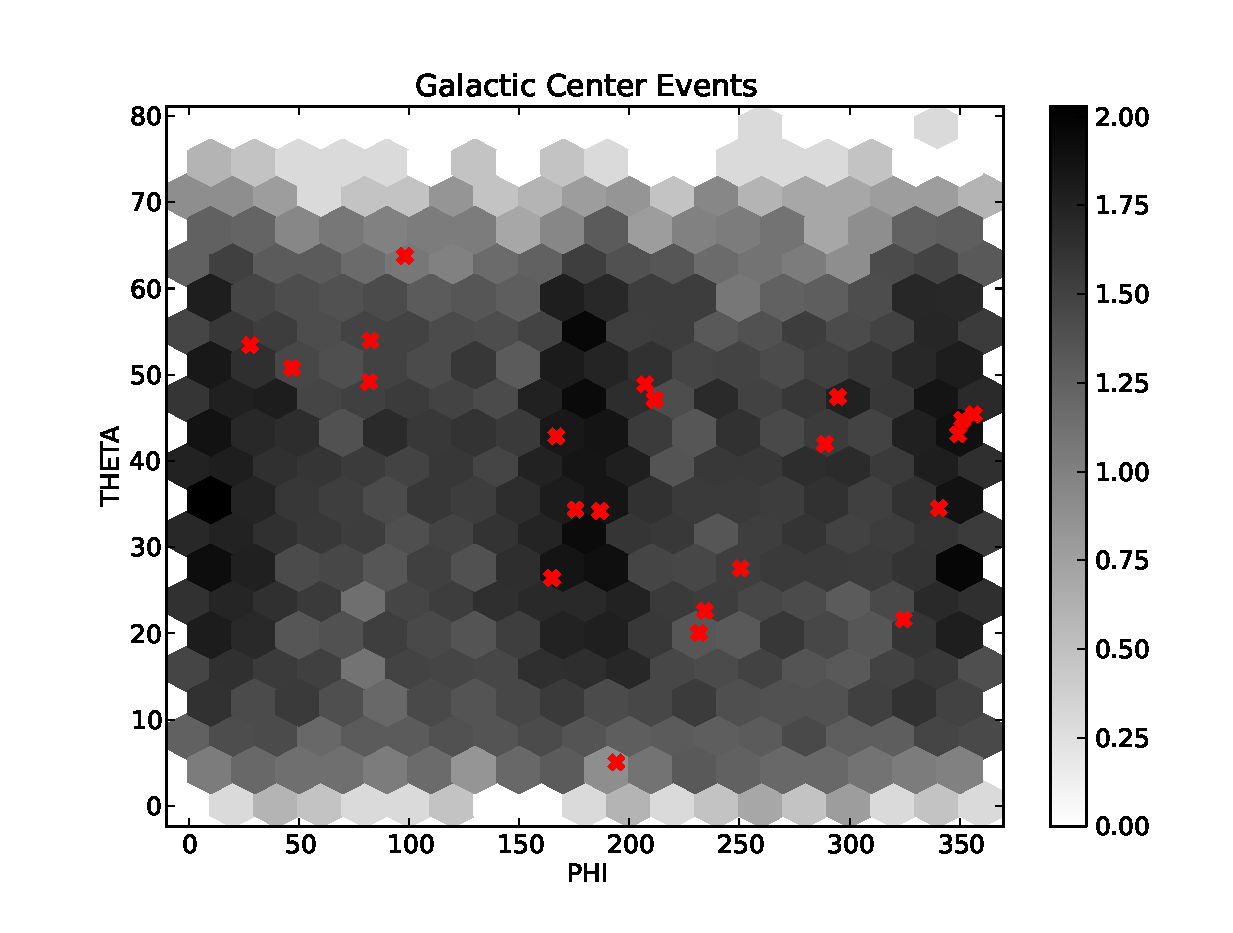
\includegraphics[width=0.48\textwidth]{plots/gc_theta_phi.eps}
%   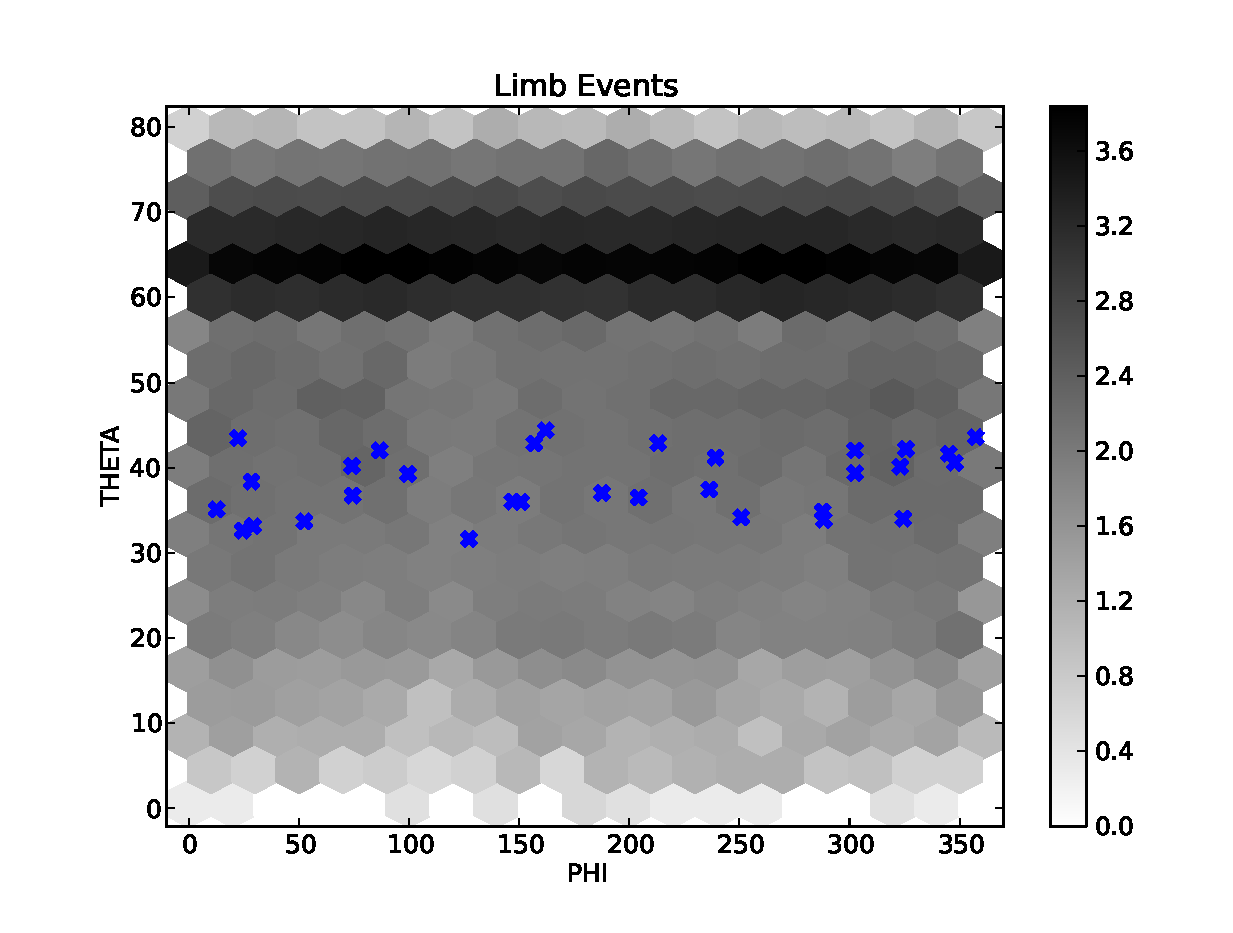
\includegraphics[width=0.48\textwidth]{plots/limb_theta_phi.eps}
%   \caption{Line events (125 GeV $< E <$ 140 GeV) in
%   physical detector angle coordinates ($\theta, \phi$).
%   The $30\degree < \theta < 45\degree$ events are blue in
%   this and following panels}
%   \label{fig:theta-phi}
% \end{figure*}
 
\begin{figure}
  \centering
  \includegraphics[width=0.9\linewidth]{plots/rockangle.ps}
  \caption{The rocking angle of the Galactic center line
  events (positive values indicate a rock angle toward the
  north from zenith)-- \textbf{need to add red and blue to
  this plot}...  }
  \label{fig:rock}
\end{figure}


\bibliography{systematics}

\end{document}
